\documentclass[a4paper, 11pt]{article}

\usepackage[utf8]{inputenc}
\usepackage{verbatim}
\usepackage{moreverb}
\usepackage[english]{babel}
\usepackage[T1]{fontenc}
\usepackage{lmodern}
\usepackage{graphicx}
\usepackage{fancyhdr}
\usepackage{listings} 
\usepackage{lastpage}
\usepackage[top=3cm, bottom=3cm, left=2cm, right=2cm]{geometry}
\usepackage{color}
\usepackage{xcolor}

%font change
\renewcommand{\familydefault}{\sfdefault}

\newcommand{\HRule}{\rule{\linewidth}{0.5mm}}
\newcommand{\nl}{\\[0.1cm]}
\newcommand{\s}{\vspace{0.3cm}}
\newcommand{\smore}{\vspace{0.6cm}}

\usepackage{caption}
\DeclareCaptionFont{white}{\color{white}}
\DeclareCaptionFormat{listing}{\colorbox{gray}{\parbox{\textwidth}{#1#2#3}}}
\captionsetup[lstlisting]{format=listing,labelfont=white,textfont=white}

\lstset{frame=single}

\lstdefinelanguage{popc}{%
   morekeywords={%
   %od
      od, url, power, @, 100, 80, machine, POPString, search
  },
  sensitive=true,
  morestring=[b]',
}

\addto\captionsenglish{%
  \renewcommand{\listfigurename}{}%
	\renewcommand\refname{}
}



%Header and footer 
\pagestyle{fancy}
\fancyhead{}
\fancyfoot{}

%Header definition
\renewcommand{\headrulewidth}{0.5pt}
\lhead{ViSaG : Virtual Safe GRID}
\rhead{Version 1.1}

%Footer definition
\renewcommand{\footrulewidth}{0.5pt}
\cfoot{\today}
\lfoot{Valentin Clément}
\rfoot{Page \thepage ~on \pageref{LastPage}}

%remove indent for paragraph
\parindent0ex 

%\setlength{\parskip2ex}








%\pagebreak



\begin{document}

% TITLE INFORMATION

\begin{titlepage}
 
\begin{center}

\includegraphics[scale=0.3]{logo_eif.png}\\[1.5cm]
\textsc{\LARGE ViSaG - Virtual Safe GRID}\\[1.5cm]


\includegraphics[scale=0.3]{pic/logo_pop.png}\\[2cm]


\HRule \\[1cm]
{ \huge \bfseries POP-C++ Virtual-Secure (VS)}\\[0.5cm]
\textsc{\LARGE POP-C++ User and Installation manual : add-on}\\[1cm]
 
\HRule \\[5cm]
 
% Author and supervisor
\begin{minipage}{0.4\textwidth}
\begin{flushleft} \large
\textbf{Author:}\\
Valentin Clément
\end{flushleft}
\end{minipage}
\begin{minipage}{0.4\textwidth}
\begin{flushright} \large
\textbf{Date:} \today \\

\textbf{Revision:} 1.0
\end{flushright}
\end{minipage}
 
\vfill
  
\end{center}
 
\end{titlepage}

%\newpage \thispagestyle{empty} \mbox{}\newpage



\tableofcontents
\pagebreak
\section{Introduction}
POP-C++ Virtual Secure (abbreviated POP-C++ VS) is a version of the POP-C++ middle-ware able to run parallel objects into virtual machines with a certain level of security for the communications between the nodes. The development of this version is the core of the ViSaG project. A prototype version of Virtual - POP-C++ has been developed during a bachelor thesis project in the summer 2010. This version is called VirtualPOPC-1\cite{vpopc1}.\s

This document is an add-on of the official POP-C++ User and Installation Manual\cite{popc_manual} to help the end user to set up a node with POP-C++ VS. \s

This document is structured as follows: 

\begin{itemize}
\item The next chapter explains the confidence link used between the nodes in a POP-C++ network. 
\item The third chapter aims to help the user to set the Admin Virtual Machine (Admin VM) and the original Worker Virtual Machine (Worker VM).
\item The fourth chapter explains the installation process of the original Worker Virtual Machine (Worker VM).
\item The fifth chapter is a glossary of the terms used in POP-C++ VS.
\end{itemize}

\section{Developer Notice}
POP-C++ VS must be used only with the Global Services. This forces tu use the resource discovery to create parallel object. We can't use object description like \textbf{od.url} as used in the POP-C++ standard version.

\section{The confidence link}

In order to be able to communicate between two POP-C++ nodes in secure mode, we need to set up the confidence link. The confidence link means that two POP-C++ nodes agree to communicate with each other with a certain level of security. \s

For the moment, the POP-C++ confidence link is set up with the exchange of the SSH Public Key. To set this confidence link between the computer A and the computer B, we should do the following actions : 

\begin{enumerate}
\item Generate the SSH Public and Private keys on each computer (command ssh-keygen). We will use the default option to generate the SSH keys. 
\item Send the SSH Public Key of A to B (use scp or another way to transfer the file from the computer A to the computer B). The SSH Public is located under \$HOME/.ssh/id\_rsa.pub
\item Send the SSH Public Key of B to A.
\item Write the SSH Public Key of A in the authorized\_keys file of B (located under \$HOME/.ssh/authorized\_keys)
\item Write the SSH Public Key of B into the authorized\_keys file of A. 
\end{enumerate}

Be sure to check your confidence link to avoid any problems during the execution of a POP-C++ application. 

\section{Set up a virtual node}
A node using POP-C++ VS is composed by minimum two virtual machines over an ESXi virtualization platform. These two virtual machines are called as follow : 

\begin{itemize}
\item \textbf{Admin VM} : This virtual machine will run the POP-C++ Global Services for the whole ESXi node. A node should have only one Admin VM (see Section \ref{lb:adminvm} to set up this VM).
\item \textbf{Worker VM} : This virtual machine will be managed by the Admin VM and will execute POP-C++ jobs (see Section \ref{lb:workervm} to set up this VM). 
\end{itemize}

The following of this chapter explains how to set up these two VM on a ESXi virtualization platform.


%--------------------
% INPUT FILE SECTION 
%--------------------
\subsection{Set up the Admin VM}
\label{lb:adminvm}
The first VM to set up in the POP-C++ VS environement is an Admin VM. The Admin VM will interact with the ESXi hypervisor to manage the Worker VM. To set up this particular VM, the following steps must be done:

\begin{itemize}
\item Install ESXi on the computer (see Appendix \ref{app:esxi})
\item Create a VM in vSphere (see Appendix \ref{app:createvm})
\item Install an OS in the created VM. 
\item Install necessary packages for POP-C++ (see Section \ref{lb:packages})
\item Configure the DNS hostname (see Section \ref{lb:dns})
\item Configure the SSH server (see Section \ref{lb:sshserver})
\item Configure, Compile and Install POP-C++ (see Section \ref{lb:popc_install})
\end{itemize}

\subsubsection{Install necessary packages for POP-C++}
\label{lb:packages}
In order to install POP-C++ VS, we need to install some additional packages. The following packages need to be installed and the default values can be used : 

\begin{enumerate}
\item libvirt 0.8.5 or later (see Appendix \ref{app:libvirt})
\item VMware tools (see Appendix \ref{app:vmwaretools})
\item VMware CLI 4.1 or later (see Appendix \ref{app:vmwarecli})
\item VIX 10.1 or later (see Appendix \ref{app:vix})
\item A C++ compiler, Zlib
\end{enumerate}

For the point 5, the following command can be used on a Debian/Ubuntu based OS.\s

\begin{lstlisting}
sudo apt-get install build-essential zlib1g-dev
\end{lstlisting}





\subsubsection{Set the ESXi DNS hostname}
\label{lb:dns}
If your network does not have a DNS server or if the hostname of the ESXi platform is not registered in it, we need to add this hostname in the host file name of the Admin VM. On a linux based OS, we will modify the file located under \textbf{/etc/hosts} and add the following line (replace with your values):\s

\begin{lstlisting}
160.98.20.140	esxivisag01.sofr.hefr.lan
\end{lstlisting}





\subsubsection{Configure SSH Server}
\label{lb:sshserver}
As the Admin VM will communicate with worker VM and these Worker will be created dynamically, we need to configure the SSH server to avoid a strict host key identification. To do that, we need to modify the file \textbf{/etc/ssh/ssh\_config} and have the following line:\s

\begin{lstlisting}
StrictHostKeyChecking no
\end{lstlisting} \s

We need to generate the SSH public/private keys to be able to run Virtual Secure POP-C++. To generate the SSH keys, we need to run the following command (use the default parameters):\s
\begin{lstlisting}
ssh-keygen
\end{lstlisting}






\subsubsection{Configure and compile POP-C++ in its Virtual Secure version}
\label{lb:popc_install}
POP-C++ needs to be configured and compiled before its installation. During the configuration, we can choose the version of POP-C++ that we want to install. For the ViSaG project, we want to install POP-C++ VS. To have this version, use the following options with the configure script: \s

\begin{lstlisting}
./configure --enable-virtual --enable-secure
\end{lstlisting}\s

\textit{NOTE:} If you already have compiled POP-C++ before, use "make clean" to clean the workspace before compiling the new version.\s

Once the configuration process is done, we can compile POP-C++. For this, use the following command: \s

\begin{lstlisting}
make
\end{lstlisting}\s

If the make command exit without errors, POP-C++ is compiled in its VS version and ready to be installed. \s

To install POP-C++, we just need to launch the following command:\s

\begin{lstlisting}
make install
\end{lstlisting}\s

The installation script will ask us some question to configure our installation. Here are the different questions and the answer we could provide:\s

\textbf{Part 1:Select the right installation}
\begin{lstlisting}
DO YOU WANT TO CONFIGURE  POP-C++ SERVICES? (y/n)
y
...
DO YOU WANT TO MAKE A SIMPLE INSTALLATION? (y/n) 
n
\end{lstlisting}\s

\pagebreak
\textbf{Part 2: Configure the parameters of the node}\\
The first question of this part asks us to enter the "full qualified master host name". This means the hostname or IP address of the node which have the confidence link with this node. 
\begin{lstlisting}
Enter the full qualified master host name (POPC gateway):

\end{lstlisting}\s

Not used in POP-C++ VS for the moment (let blank)
\begin{lstlisting}
Enter the child node:

\end{lstlisting}\s

Enter the number of processors available on the whole node. 
\begin{lstlisting}
Enter number of processor available (default:1):

\end{lstlisting}\s

Set the number of jobs that can be concurrently executed on the node for all VM.
\begin{lstlisting}
Enter the maximum number of POP-C++ jobs that can run concurrently 
(default:100):
20
\end{lstlisting}\s

Set the available RAM for the whole node.
\begin{lstlisting}
Enter the available RAM for job execution in MB (default: 1024):
4096
\end{lstlisting}\s

Set the user you want to use to execute the jobs (usually the same as the one who installed POP-C++, let blank)
\begin{lstlisting}
Which local user you want to use for running POP-C++ jobs?

\end{lstlisting}\s


\begin{lstlisting}
CONFIGURE THE RUNTIME ENVIRONMENT
Enter the script to submit jobs to the local system:

Communication pattern:

\end{lstlisting}\s

\pagebreak
\textbf{Part3: Setting up the virtual environment}\\
It's time to set up the virtual environment for POP-C++. We need the information about the ESXi platform and the worker VM. If the worker VM is not set up yet, these information can be edited later in the file POPC\_LOCATION/etc/virtual.conf.
\begin{lstlisting}
SETTING UP VIRTUAL ENVIRONMENT INFORMATION NOW
ESX(i) hypervisor IP address : e.g. 160.98.20.140
160.98.20.141
ESX(i) user name with admin rights (default: root)
root
ESX(i) password:
*****
ESX(i) datastore name (default: datastore1)

ESX(i) maximum worker (default: 4)

ESX(i) worker name (default: popc_worker_guest1)
visag04_worker1
ESX(i) worker OS username
visag
ESX(i) worker OS password
*****
ESX(i) clean snapshot name (default: popc_clean)
popc_clean
\end{lstlisting}\s





\textbf{Part 4: runtime environment variables}\\
We can set up some environment variables to be used in the runtime of POP-C++. No particular variables needs to be set for POP-C++ VS.
\begin{lstlisting}
SETTING UP RUNTIME ENVIRONMENT VARIABLES
Enter variable name:

Enter variable value:

\end{lstlisting}\s

\pagebreak
\textbf{Part 5: Installation end}\\
It's important to generate the startup script because it will be used to run the POP-C++ Global Services on the Admin VM.
\begin{lstlisting}
===============================
CONFIGURATION POP-C++ SERVICES COMPLETED
===============================
Do you want to generate the POP-C++ startup scripts? (y/n)
y
Enter the service port[2711]:

Enter the domain name:

Enter the temporary directory for intermediate results:

===============================
CONFIGURATION DONE!
===============================

IMPORTANT : Do not forget to add these lines to your .bashrc file or 
equivalent:

POPC_LOCATION=/home/visag/popc
PATH=$PATH:$POPC_LOCATION/bin:$POPC_LOCATION/sbin
\end{lstlisting}\s




\subsubsection{Run the POP-C++ services on the Admin VM}
After the preparation and installation of POP-C++ VS on the Admin VM, we can now start the Global Services on the node. Use this command to start the POP-C++ Global Services : 
\begin{lstlisting}
SXXpopc start
\end{lstlisting}\s

You will see the followings lines if the startup is successful (the IP addresses and ports will be different):\s
\begin{lstlisting}
Starting POP-C++ [Virtual Secure Version] Global Services
VSPSN Started [socket://160.98.21.195:49391]
VPSM Started [socket://160.98.21.195:37958]
POPCloner Started [socket://160.98.21.195:52035]
VSJM created [socket://160.98.21.195:2711]
\end{lstlisting}\s

If an exception occurs at start up, please check one of the following log files to find the problem: 

\begin{itemize}
\item /tmp/popc\_node\_log
\item /tmp/popc\_security\_log
\item /tmp/popc\_clone\_log
\end{itemize}

\textit{NOTE:} The /tmp directory is the default log files directory you may have changed it with another directory
 

\pagebreak
\subsection{Set up the original Worker VM}
\label{lb:workervm}
As POP-C++ VS will clone workers as needed, we just need to set up the first "original" Worker VM. To set this particular worker VM, the following steps must be done : 

\textbf{\textit{WARNING:}} Read carfully the restriction imposed to the name, username and password. These restrictions are strict and cannot be worked around. 
\begin{itemize}
\item Create VM in vSphere (see Appendix \ref{app:createvm}). The VM name \textbf{must} have the suffix \textbf{\_worker1} (other suffixes are not supported for the moment).
\item Install an OS on the create VM.
\item Install necessary packages for POP-C++ (see Section \ref{lb:workerpackages})
\item Install VMware tools on the worker VM (see Appendix \ref{app:vmwaretools})
\item Configure SSH for the worker VM (see Section \ref{lb:workerssh})
\item Configure, Compile and Install POP-C++ Standard (see Section \ref{lb:workerpopc})
\item Create a snapshot of the worker VM (see Appendix \ref{app:snap})
\end{itemize}


\subsubsection{Necessary packages}
\label{lb:workerpackages}
To be able to run application using POP-C++ VS on the worker VM, we need to install some packages. Here are the list of the needed packages : 

\begin{itemize}
\item A C++ compiler
\item An SSH server
\item Zlib compression library
\end{itemize}

On a Debian/Ubuntu based OS, we can use the following command to install those packages.\s

\begin{lstlisting}
sudo apt-get install build-essential openssh-server zlib1g-dev
\end{lstlisting}

\subsubsection{Configure SSH server on the worker VM}
\label{lb:workerssh}
As POP-C++ VS uses the secure mode of POP-C++ to communicate between the nodes, we need to set up the SSH parameters. First, we need to generate the SSH public/private keys pair. Use the following command and keep the default values.\s

\begin{lstlisting}
ssh-keygen
\end{lstlisting}\s

We also need to let the SSH server accept host key without a strict check. For this, we need to modify the file \textbf{/etc/ssh/ssh\_config} and have the following line : \s

\begin{lstlisting}
StrictHostKeyChecking no
\end{lstlisting}

\subsubsection{Configure, Compile and Install POP-C++}
\label{lb:workerpopc}
On the Worker VM, we just need a standard version of POP-C++. Here are the commands to execute to configure and compile POP-C++ in its standard version.\s
\begin{lstlisting}
./configure
make
\end{lstlisting}

Once POP-C++ is compiled, we can install it. Use the following command : \s

\begin{lstlisting}
make install 
...
DO YOU WANT TO CONFIGURE  POP-C++ SERVICES? (y/n)
y
DO YOU WANT TO MAKE A SIMPLE INSTALLATION? (y/n) 
y
...
===============================
CONFIGURATION DONE!
===============================

IMPORTANT : Do not forget to add these lines to your .bashrc file or 
equivalent:

POPC_LOCATION=/home/visag/popc
PATH=$PATH:$POPC_LOCATION/bin:$POPC_LOCATION/sbin
\end{lstlisting}

\textit{NOTE:} Don't forget to add the lines in your .bashrc or equivalent file if you changed the default installation location otherwise the node will not run normally.

\section{Compatibility issues}
\label{lb:compatibility}
As POP-C++ can be compiled in 4 different versions, there are some compatibility issues between those versions. The table below indicates which version can be used together.

\begin{center}
\begin{tabular}{|p{3cm}|p{3cm}|p{3cm}|p{3cm}|p{3cm}|}
\hline
\textbf{Version/Version} & \textbf{Standard}	& \textbf{Secure} & \textbf{Virtual} & \textbf{Virtual-Secure}\\ \hline
\textbf{Standard} & \textcolor{green}{OK} & \textcolor{red}{NO OK} & \textcolor{green}{OK} & \textcolor{red}{NO OK} \\ \hline
\textbf{Secure} & \textcolor{red}{NO OK} & \textcolor{green}{OK} & \textcolor{red}{NO OK} & \textcolor{green}{OK} \\ \hline
\textbf{Virtual} & \textcolor{green}{OK} & \textcolor{red}{NO OK} & \textcolor{green}{OK} & \textcolor{red}{NO OK} \\ \hline
\textbf{Virtual-Secure} & \textcolor{red}{NO OK} & \textcolor{green}{OK} & \textcolor{red}{NO OK} & \textcolor{green}{OK} \\ \hline
\end{tabular}
\end{center}\s

\textit{NOTE:} Be aware that an application compiled with POP-C++ Secure or Virtual-Secure will not run with POP-C++ Standard or Virtual. You need to recompile the application before running it.


\section{Functional test procedure}
This chapter will help you to set up an infrastructure with one or several POP-C++ node and test it. 


\subsection{Test a single node}
The first thing to test is the single node installation. This test is done just to make sure that the Admin VM and the Worker VM are configured correctly to work together. \s

\textbf{Start the Global Services on the Admin VM}\\
First we need to start the POP-C++ Global Services on the Admin VM to be able to run a POP-C++ application. For this, use the following command:\s

\begin{lstlisting}
SXXpopc start
\end{lstlisting}\s

You should have a result as follows: \s

\begin{lstlisting}
Starting POP-C++ [Virtual Secure Version] Global Services
VSPSN Started [socket://160.98.21.238:54314] 
VPSM Started [socket://160.98.21.238:44603] 
POPCloner Started [socket://160.98.21.238:34485] 
VSJM Started [socket://160.98.21.238:2711] 
\end{lstlisting}\s

If you already have an error at this step, check the virtual configuration file located under \textit{POPC\_LOCATION} /etc/virtual.conf and be sure to have set the right parameters for your ESXi hypervisor and VMs.\s

Once the POP-C++ Global Service are started, we are ready to run a POP-C++ application on the node. For this, go to \textit{POPC\_RELEASE\_FOLDER}/demos/demopopc. We need to compile the code.\s

\begin{lstlisting}
make
\end{lstlisting}\s

Once the code is compiled, we need to provide a way to find this executable code. The easiest way is to put the code on a Web Server or FTP Server. The second way is to have a NFS. But for the second solution, we have to configure the Admin VM and Worker VM with the same NFS.\s

The most important is that the Worker VM can download the code to execute it. In our demo example, the code is \textbf{demopopc.obj}. This file must be accessible for the Worker VM. \s

Once the executable is accessible from somewhere, we need to edit the object map file. In our example, this file is named \textbf{obj.map}. Depending on the architecture, and location of the executable, this file could look like this. \s
\begin{lstlisting}
POPCobject i686-pc-Linux http://www.popcwebserver.com/example1/demoobj.obj
\end{lstlisting}


% #############################
% MULTIPLE NODES TEST
% #############################

\pagebreak
\subsection{Test several node}
To test the execution on several nodes, we first need to set up an infrastructure of POP-C++ nodes. We will set up 3 POP-C++ nodes to test two different aspects of POP-C++ VS.


%
% REFERENCE PASSING TEST
%
\subsubsection{Object reference passing test}

\textbf{Infrastructure schema}\\
Here is the connection schema of the infrastructure we would like to test. It's important to have two node that doesn't know each other. 
\begin{figure}[ht]
	\caption{Test Case 1: Logical Connection}
  	\centering
	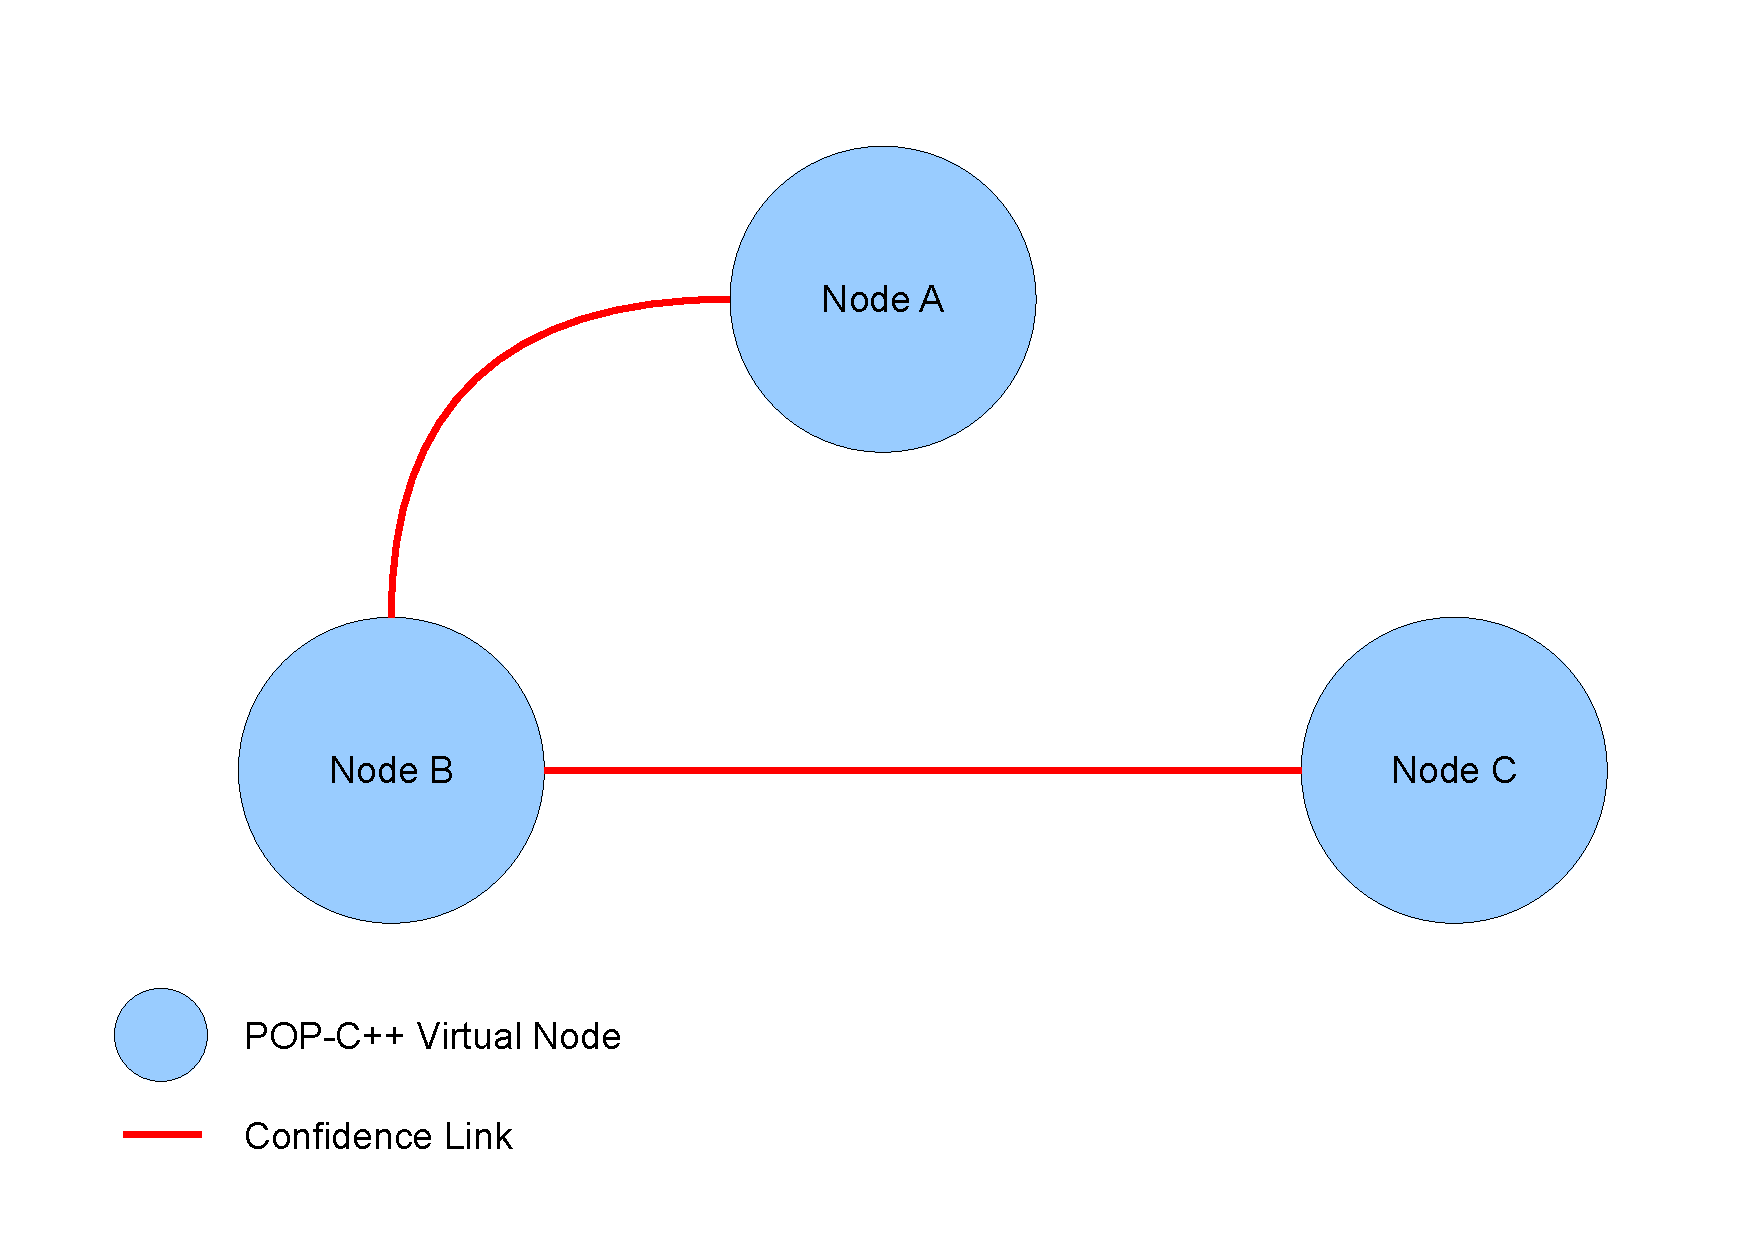
\includegraphics[width=0.7\textwidth]{./pic/testcase2.pdf}
	\label{fig:testcase1}
\end{figure}

\textbf{Infrastructure configuration}\\
\begin{itemize}
\item Node A has no master nodes. Node A has the PKI of Node B. The number of job is limited to 1 during the installation.
\item Node B has Node A as master node. Node B has the PKI of Node A and Node C. The number of job is limited to 1 during the installation.
\item Node C has Node B as master node. Node C has the PKi of Node B. The number of job is limited to 2 during the installation.
\end{itemize}
The Node A must be started first, Node B second and Node C after. \s


\textbf{Compilation and execution of test program}\\
To test this specific case, we will use the program located under \textit{POPC\_RELEASE\_FOLDER}/example/ multiobj/. To compile  this program, use the following command:\s

\begin{lstlisting}
make
\end{lstlisting}\s

As for the single node test, we need to provide a way to find the executable code. The file "demopopc.obj" must be uploaded on a Web or FTP server or located on a NFS drive. Once the file is accessible by and VM in the network, we must edit the obj.map file. Here is a sample of this file. \s
\begin{lstlisting}
POPCobject i686-pc-Linux http://www.popcwebserver.com/example1/demoobj.obj
\end{lstlisting}\s


Once the program is compiled and the executable accessible, use this command to run the program:\s
\begin{lstlisting}
popcrun obj.map ./main
\end{lstlisting}\s

Three Worker VM must be started on the three nodes. The program should end successfully. 


%
% DECENTRALIZED CREATION TEST
%

\subsubsection{Decentralized object creation test}
In this first test, we will check the creation of object by different nodes. \s

\textbf{Infrastructure schema}\\
Here is the connection schema of the infrastructure we would like to test. It's important to have one node between the first node (Main Node) and the last node. 
\begin{figure}[ht]
	\caption{Test Case 2: Logical Connection}
  	\centering
	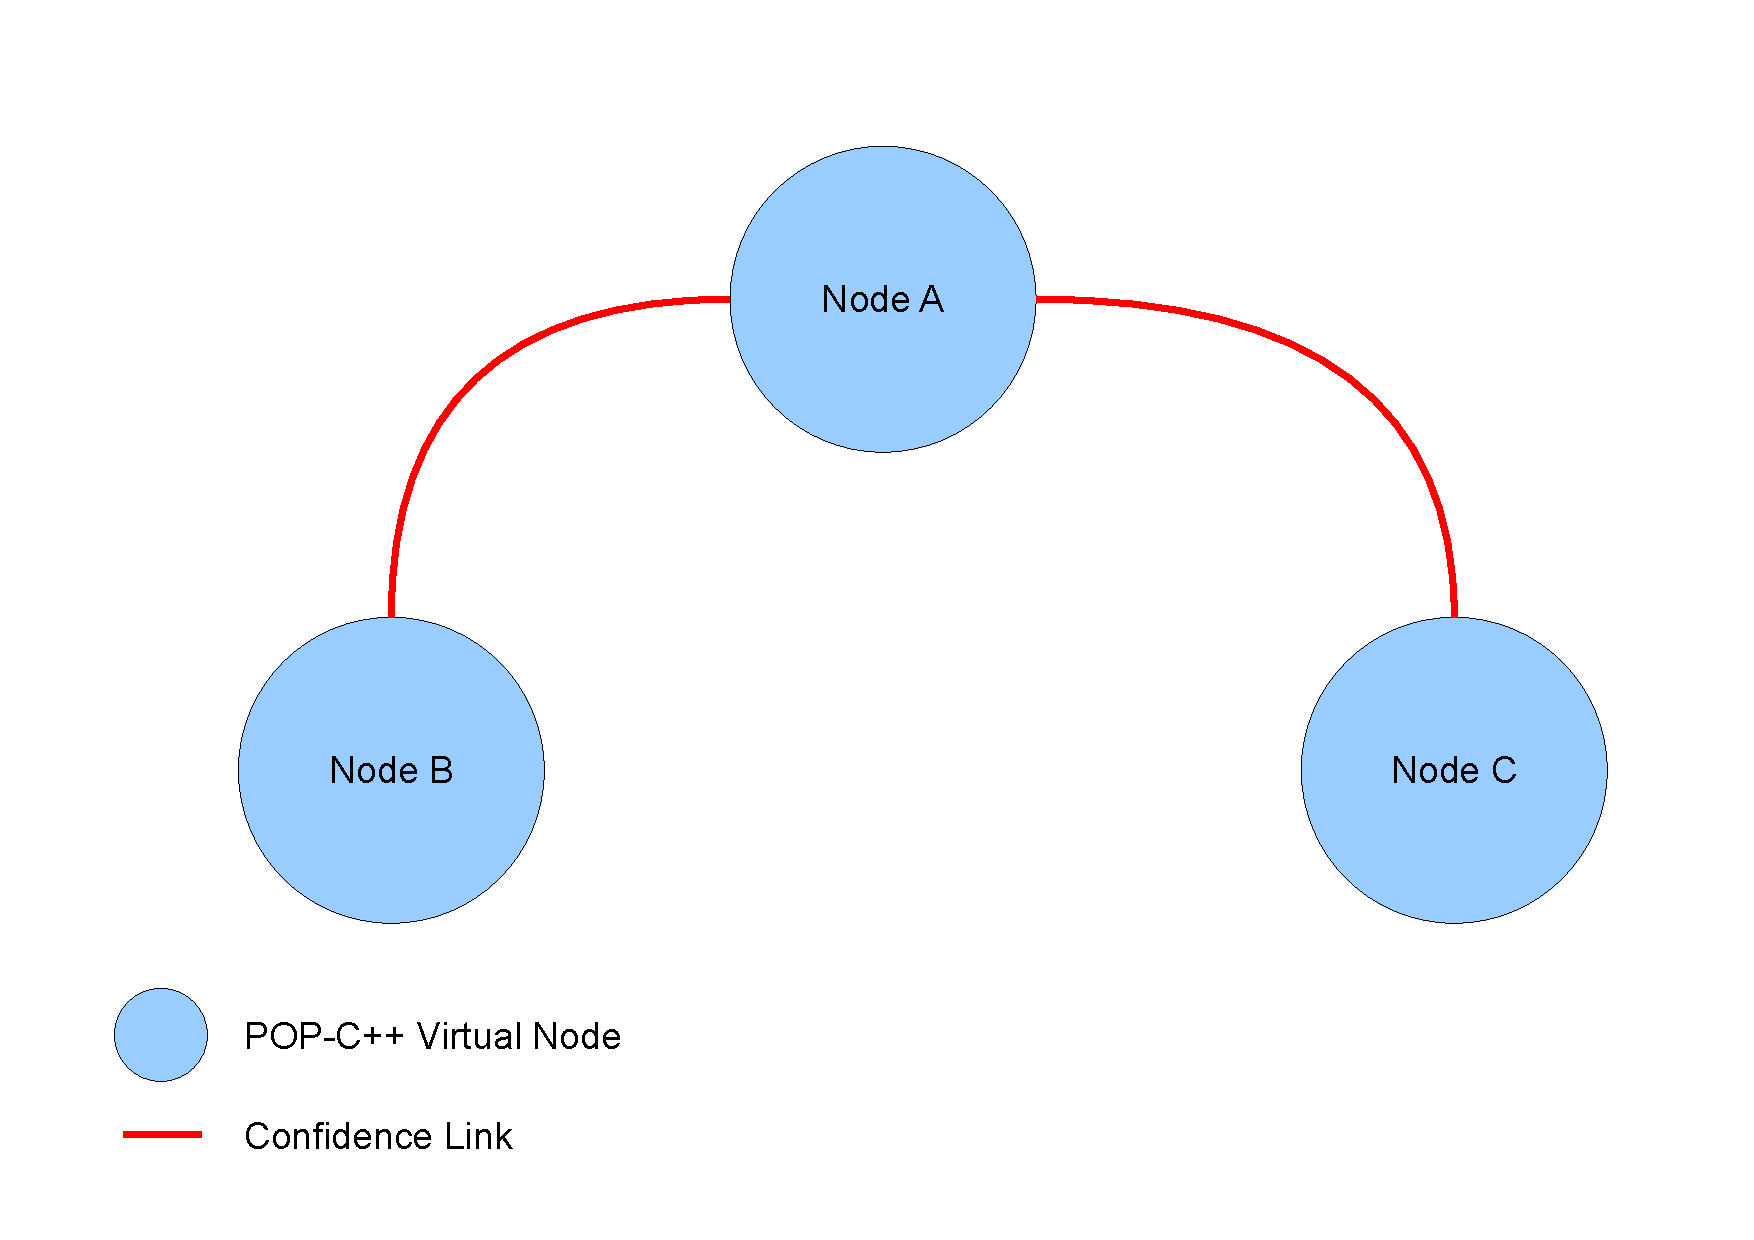
\includegraphics[width=0.7\textwidth]{./pic/testcase1.pdf}
	\label{fig:testcase1}
\end{figure}

\textbf{Infrastructure configuration}\\
\begin{itemize}
\item Node A has no master nodes. Node A has the PKI of Node B and Node C. The number of job is limited to 1 during the installation.
\item Node B has Node A as master node. Node B has the PKI of Node A. The number of job is limited to 1 during the installation.
\item Node C has Node A as master node. Node C has the PKi of Node A. The number of job is limited to 1 during the installation.
\end{itemize}
The Node A must be started first and Node B and C after. \s

\textbf{Compilation and execution of test program}\\
To test this specific case, we will use the program located under \textit{POPC\_REALEASE\_FOLDER}/demos/ demopopc/. To compile this program, use the following command:\s

\begin{lstlisting}
make
\end{lstlisting}\s

Once the program is compiled, use this command to run the program:\s
\begin{lstlisting}
popcrun objmap ./main 3 - - -
\end{lstlisting}\s

Three Worker VM must be started on the three nodes. The program should end successfully. 




\subsection{Test conclusion}
If the three tests have been executed successfully, we are now sure that our POP-C++ infrastructure is ready to execute our own program.







\section{New options}
The SXXpopc has two new options. The first one is "kill" to kill all the POP-C++ Global Services. The second one is "vmstate" to give the state of the VM on a specific node. \s

\textbf{kill}\\
The option "kill" does not take any parameters:
\begin{lstlisting}
SXXpopc kill
\end{lstlisting}\s

\textbf{vmstate}\\
The option "vmstate" takes three parameters: 
\begin{itemize}
\item IP address: The IP address of the ESXi hypervisor
\item Username: The username used to connect to the hypervisor
\item Password: The password use to connect to the hypervisor
\end{itemize}

\begin{lstlisting}
SXXpopc vmstate 160.98.20.142 root myPassword
\end{lstlisting}



\pagebreak
\section{Glossary}

\begin{itemize}
\item \textbf{POP-C++} : refers to POP-C++ in general or to the standard version of POP-C++.
\item \textbf{POP-C++ S} : refers to POP-C++ Secure version.
\item \textbf{POP-C++ V} : refers to POP-C++ Virtual version.
\item \textbf{POP-C++ VS} : refers to POP-C++ Virtual-Secure version.
\item \textbf{Admin VM} : refers to the Admin Virtual Machine managing the POP-C++ Virtual Node.
\item \textbf{Worker VM} : refers to the Worker Virtual Machine managed by the Admin VM.
\item \textbf{PSN} : POP-C++ Search Node.
\item \textbf{VPSN} : Virtual POP-C++ Search Node.
\item \textbf{SPSN} : Secure POP-C++ Search Node.
\item \textbf{VSPSN} : Virtual Secure POP-C++ Search Node.
\item \textbf{PSM} : POP-C++ Security Manager.
\item \textbf{VPSM} : Virtual POP-C++ Security Manager.
\item \textbf{JM} : Job Manager.
\item \textbf{VJM} : Virtual Job Manager.
\item \textbf{SJM} : Secure Job Manager.
\item \textbf{VSJM} : Virtual Secure Job Manager.
\end{itemize}

\pagebreak
\section{Table of figures}
\listoffigures{}

%
% 
%

\section{References}
\begin{thebibliography}{9}
\bibitem{vpopc1}
	Adrian Wyssen,
  	\emph{VirtualPOPC-1 : Project Report}.
	EIA-FR, Switzerland, 
	June-August 2010.
	
\bibitem{popc_manual}
	The POP-C++ Team,
  	\emph{Parallel Object Programming C++, User and installation Manual}.
	Grid and Cloud Computing Group, EIA-FR, Fribourg, Switzerland, 
	2010.
	
\bibitem{popcssh}
	Valentin Clément,
	\emph{POP-C++ over SSH Tunnel}.
	EIA-FR, Switzerland,
	September-November 2010.

\end{thebibliography}


%-- APPENDIX

\pagebreak
\appendix
%---------------
% LIBVIRT INSTALL
%---------------

\section{libvirt 0.8.7 installation}
\label{app:libvirt}
POP-C++ Virtual Secure uses libvirt to interact with the ESXi platform. We need to install libvirt before compiling and installing POP-C++. \s

The latest version of libvirt is available at : http://www.libvirt.org\s

To install libvirt, we need first to install some packages. On a Debian/Ubuntu Os we can use apt-get to install the following packages: \s

\begin{lstlisting}
sudo apt-get install libxml2 libxml2-dev libgnutls-dev libdevmapper-dev 
libcurl4-openssl-dev libvirt-dev libnl-dev
\end{lstlisting}\s

After the installation of these packages, we need to install the libvirt distribution downloaded from the official libvirt website. To configure libvirt with the ESXi driver use the following command: \s

\begin{lstlisting}
./configure --with-esx=yes
\end{lstlisting}\s

We can make sure that the ESX driver support is enabled by checking the end of the configure script output. We should have the following line:\s

\begin{lstlisting}
configure: ESX: yes
\end{lstlisting}\s

Once the configure process is done, we can compile and install libvirt. Use the following commands to do that. \s

\begin{lstlisting}
make 
sudo make install
\end{lstlisting}



%---------------
% VMWARE TOOLS INSTALL
%---------------
\pagebreak
\section{VMware Tools 8.3.2 installation}
\label{app:vmwaretools}
To install the latest VMware tools on the VM, we need to use the vSphere Client. On the left side, we need to right-click on the VM and select Guest > Install/Upgarde VMware Tools (see Figure \ref{fig:vmwaretoolsinstall1}). This action will connect a virtual CD-ROM on the VM. 

\begin{figure}[ht]
	\caption{VMware Tools Install (Step 1) }
  	\centering
	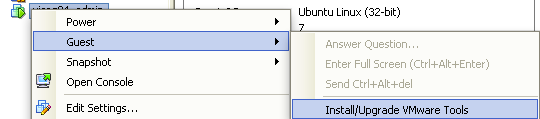
\includegraphics[width=0.5\textwidth]{./pic/vmwaretools_1.png}
	\label{fig:vmwaretoolsinstall1}
\end{figure}

Once the CD-ROM is connected to the VM, we need to mount it. Use the following command to mount it and to launch the installation process. We do a default installation. \s

\begin{lstlisting}
sudo mount /dev/cdrom /media/cdrom
cp /media/cdrom/VMwareTools-8.3.2-257589.tar.gz ./
tar -xvf VMwareTools-8.3.2-257589.tar.gz
cd vmware-tools-distrib
sudo ./vmware-install.pl
\end{lstlisting}




%---------------
% VMWARE CLI INSTALL
%---------------

\section{VMware CLI 4.1 installation}
\label{app:vmwarecli}

The VMware CLI are used by POP-C++ to do some action that are not currently possible with libvirt such as the cloning process. \s

The latest version of the VMware CLI can be found at : http://www.vmware.com/support/developer/vcli/ \s

To install the VMware CLI, we need first to install some packages. On a Debian/Ubuntu Os we can use apt-get to install the following packages: \s

\begin{lstlisting}
sudo apt-get install libcrypt-ssleay-perl libssl-dev libxml-libxml-perl
\end{lstlisting}

After the installation of these packages, we can install the VMware CLI itself. To do it, use the following commands:\s

\begin{lstlisting}
tar -xvf VMware-vSphere-CLI-4.1.0-254719.i386.tar.gz
cd vmware-vsphere-cli-distrib
sudo ./vmware-install.pl
\end{lstlisting}\s

Just follow the installation script and enter default values. 




%---------------
% VIX INSTALL
%---------------
\pagebreak
\section{VIX 1.10.2 installation}
\label{app:vix}
The VMware VIX API is used by POP-C++ for some action that are not currently available in libvirt such as sending file to a VM or executing command on VM.\s

The latest version of VIX can be found at : http://www.vmware.com/support/developer/vix-api/

To install the VIX API, we just run the bundle with the following command: \s

\begin{lstlisting}
sudo sh VMware-VIX-1.10.2-331863.i386.bundle
\end{lstlisting}



%---------------
% ESXI INSTALL
%---------------
\section{VMware ESXi 4.1}
\label{app:esxi}
The first step is to install the ESXi hypervisor on your hardware if it's not done already. Be sure that your hardware is listed in the "Hardware Compatibility Guide" (http://www.vmware.com/resources/compatibility/search.php). \s

The latest version of VMware ESXi can be found at: http://www.vmware.com/products/vsphere-hypervisor/

\textbf{Step 1:}\\
We first need a bootable CD-ROM of ESXi 4.1 or later. Once the CD-ROM is in the computer and the computer is started, the "VWware ESXi Boot Menu" will appear. At this step, we need to choose to boot from the ESXi Installer. 

\begin{figure}[ht]
	\caption{VMware ESXi Boot Menu}
  	\centering
	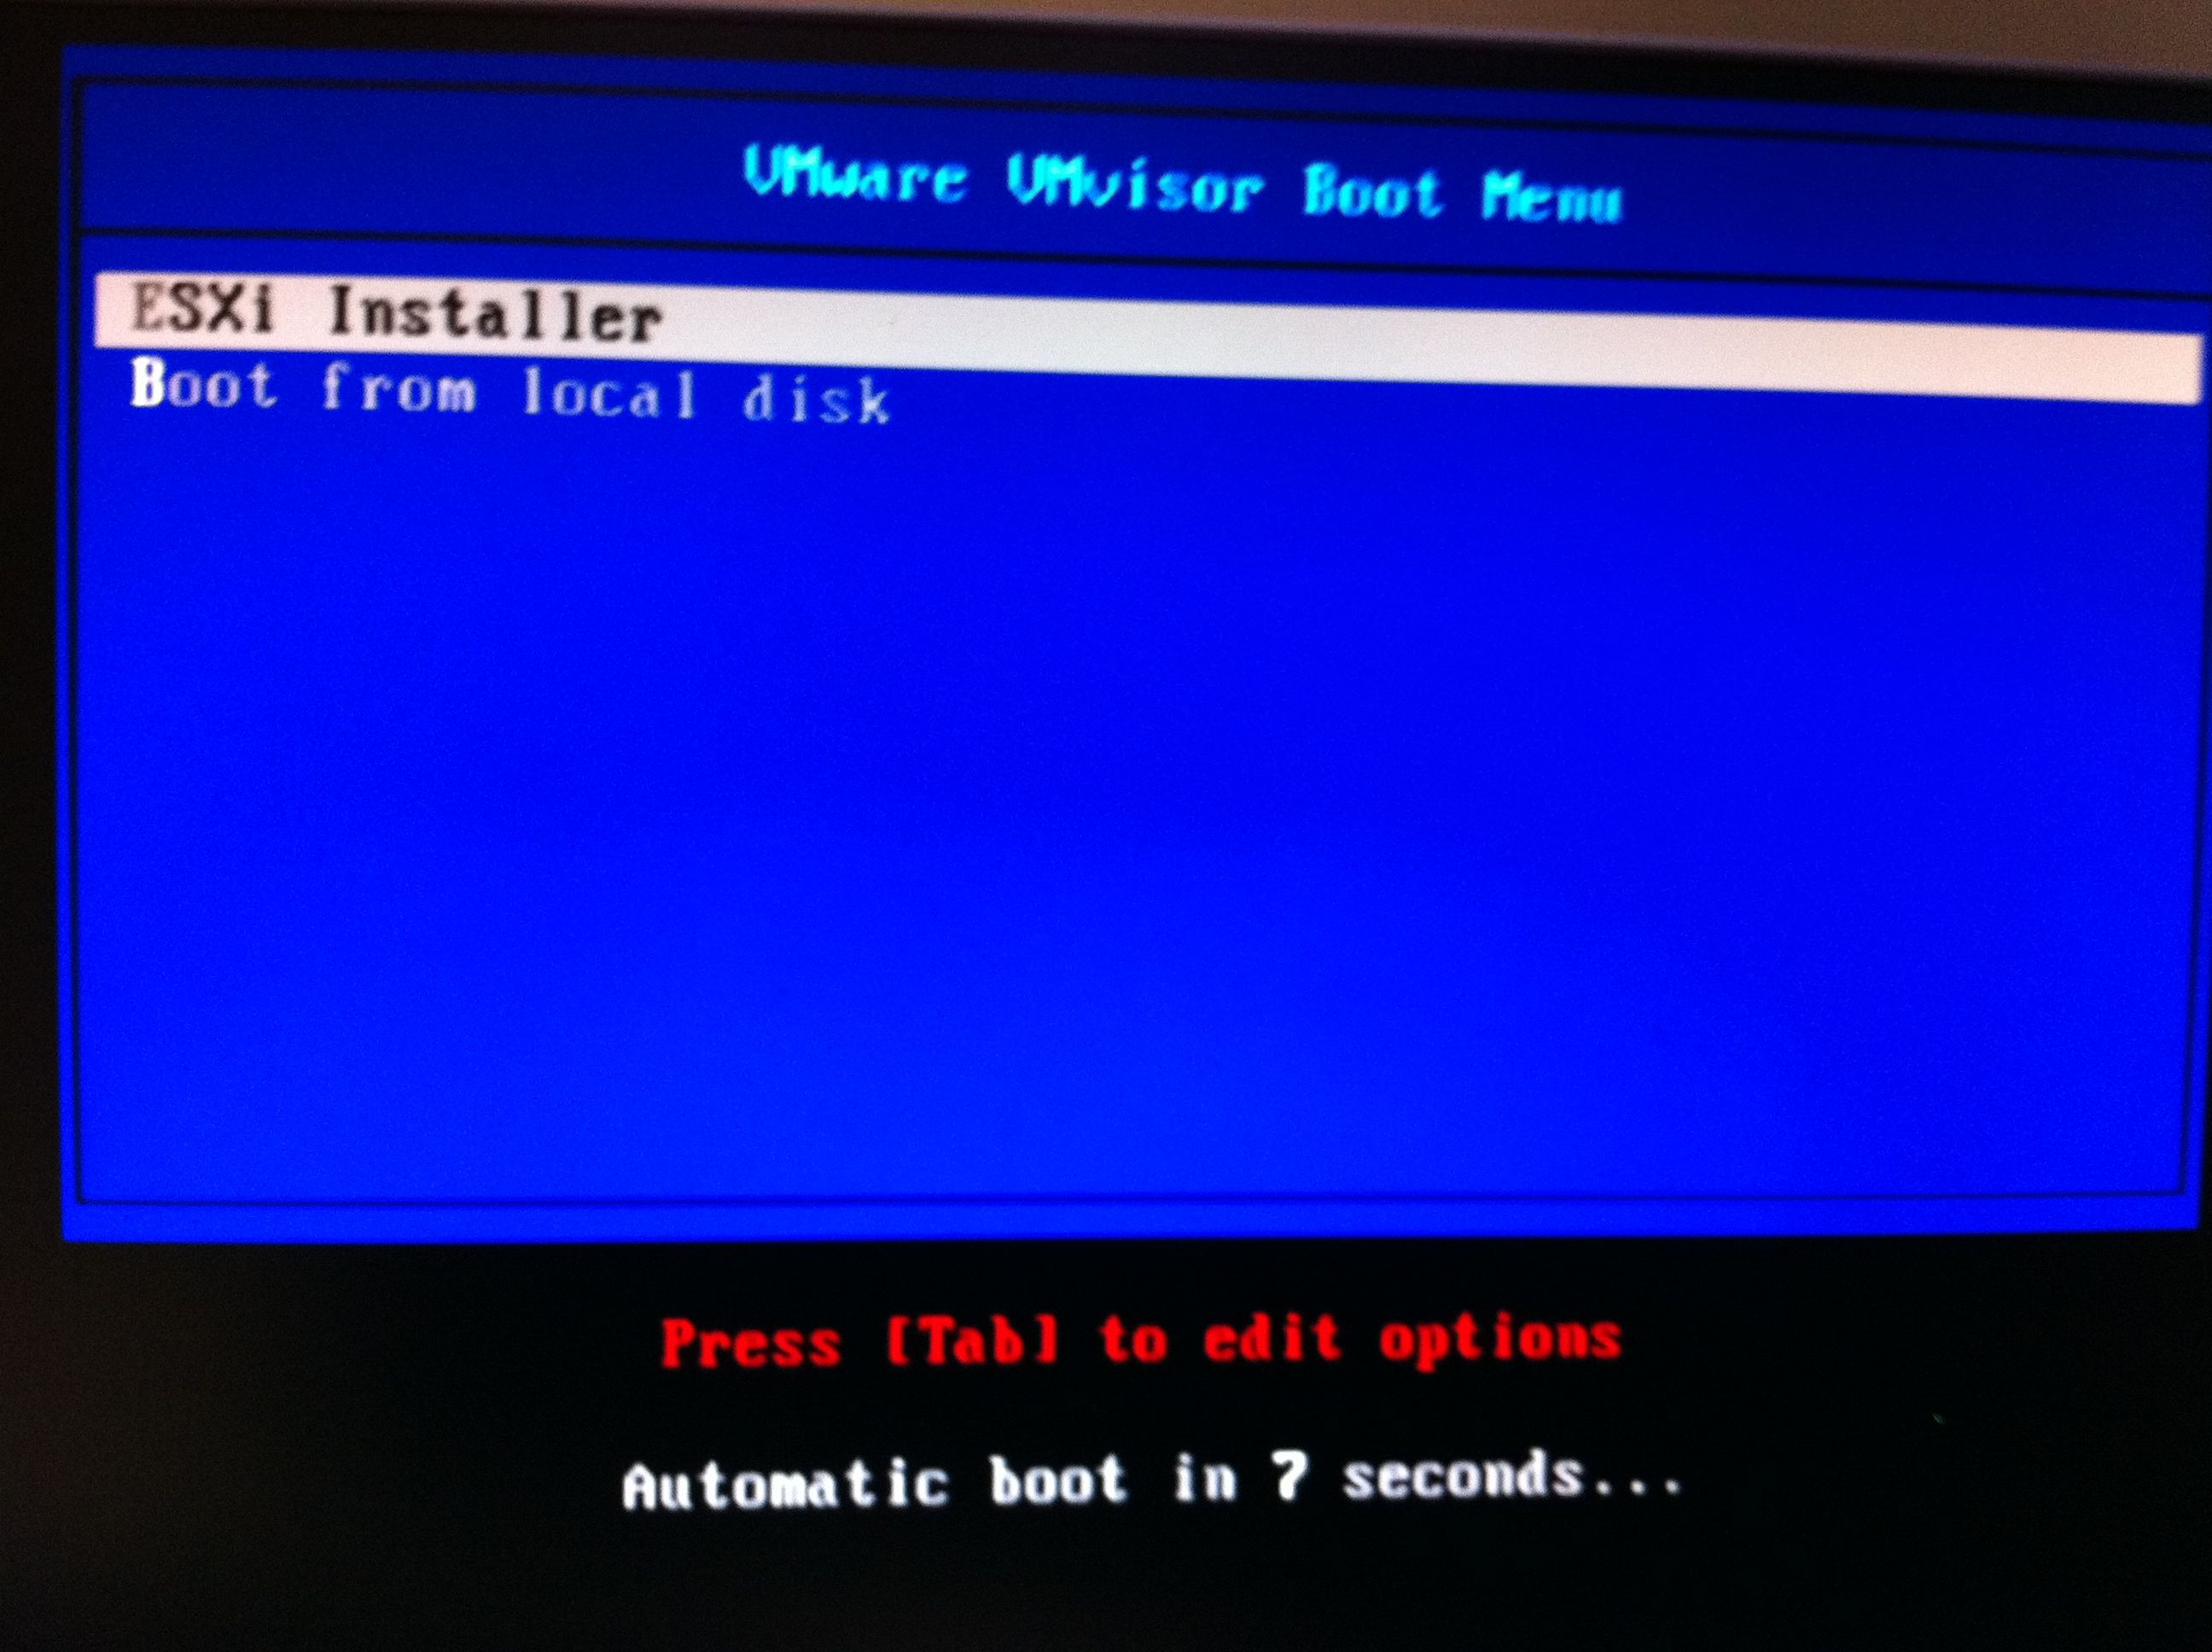
\includegraphics[width=0.5\textwidth]{./pic/esxi_1.jpg}
	\label{fig:kex_object_creation}
\end{figure}

\textbf{Step 2:}\\
Once the installer has started, the welcome screen will be displayed. On this screen, we would choose the "Install" option by pressing the "Enter" key. 

\begin{figure}[ht]
	\caption{VMware ESXi Installation Welcome screen}
  	\centering
	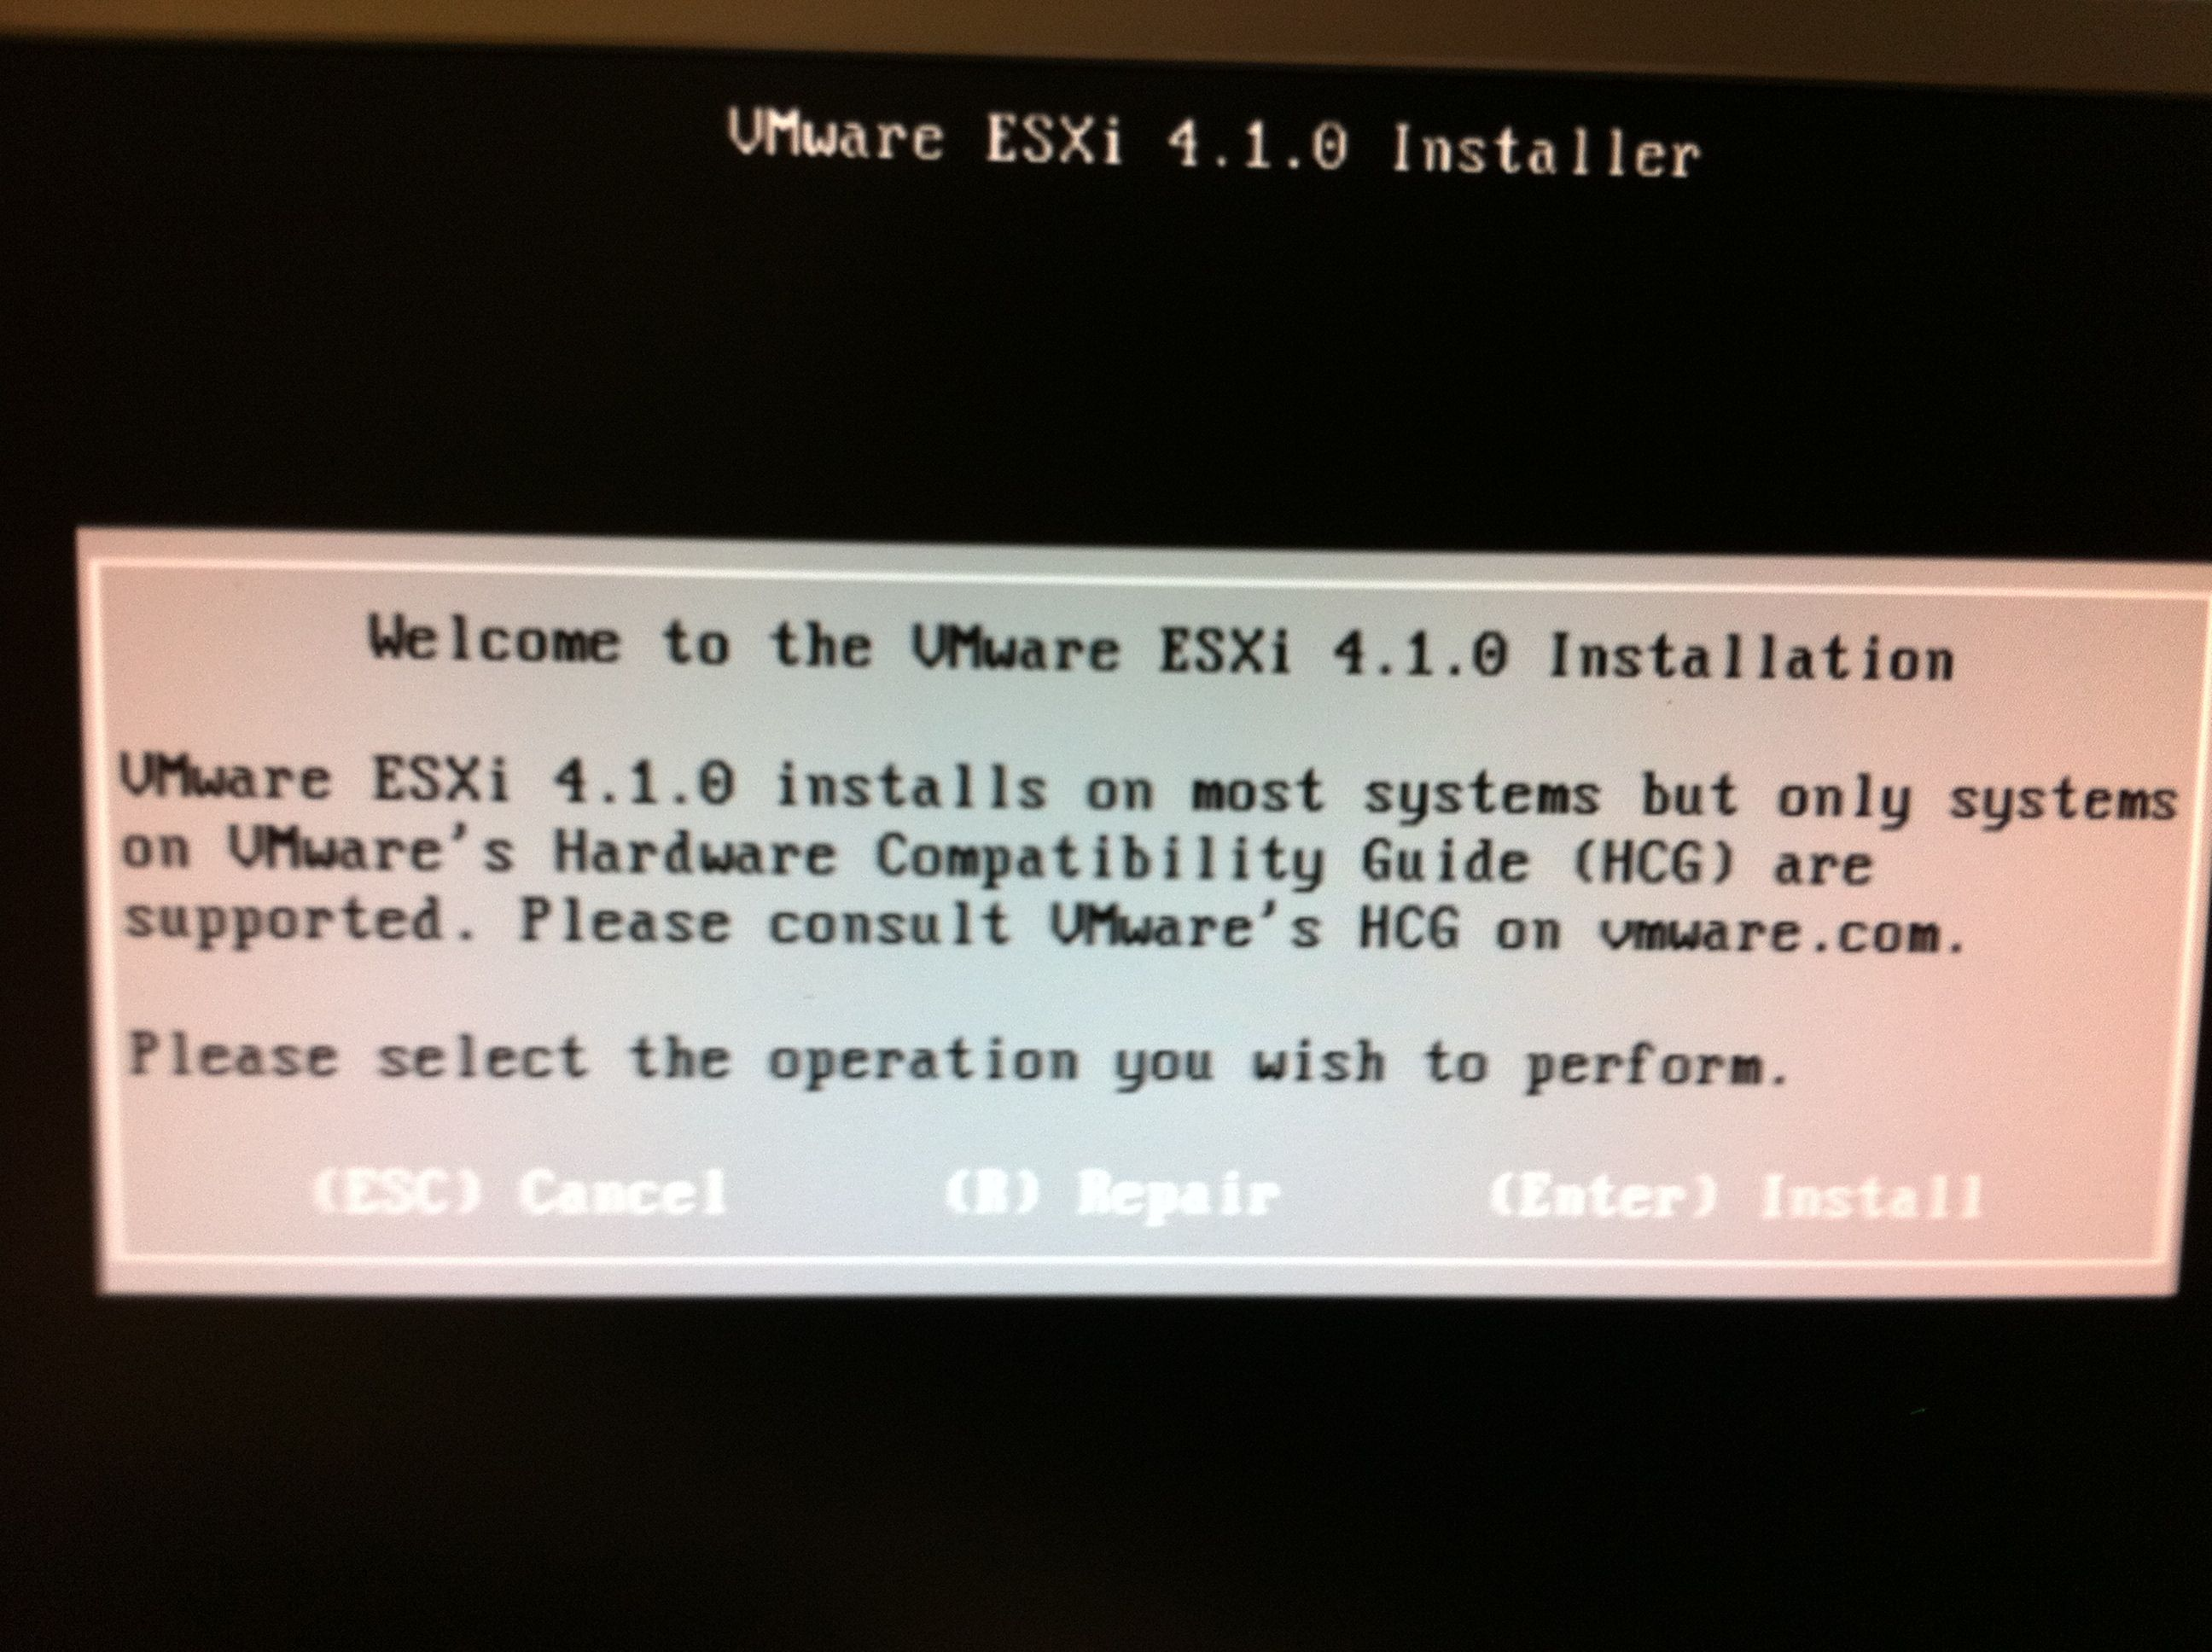
\includegraphics[width=0.5\textwidth]{./pic/esxi_2.jpg}
	\label{fig:kex_object_creation}
\end{figure}

\pagebreak
\textbf{Step 3:}\\
We will need to agree the licence of VMware ESXi by pressing the "F11" key. 
\begin{figure}[ht]
	\caption{VMware ESXi licence agreement}
  	\centering
	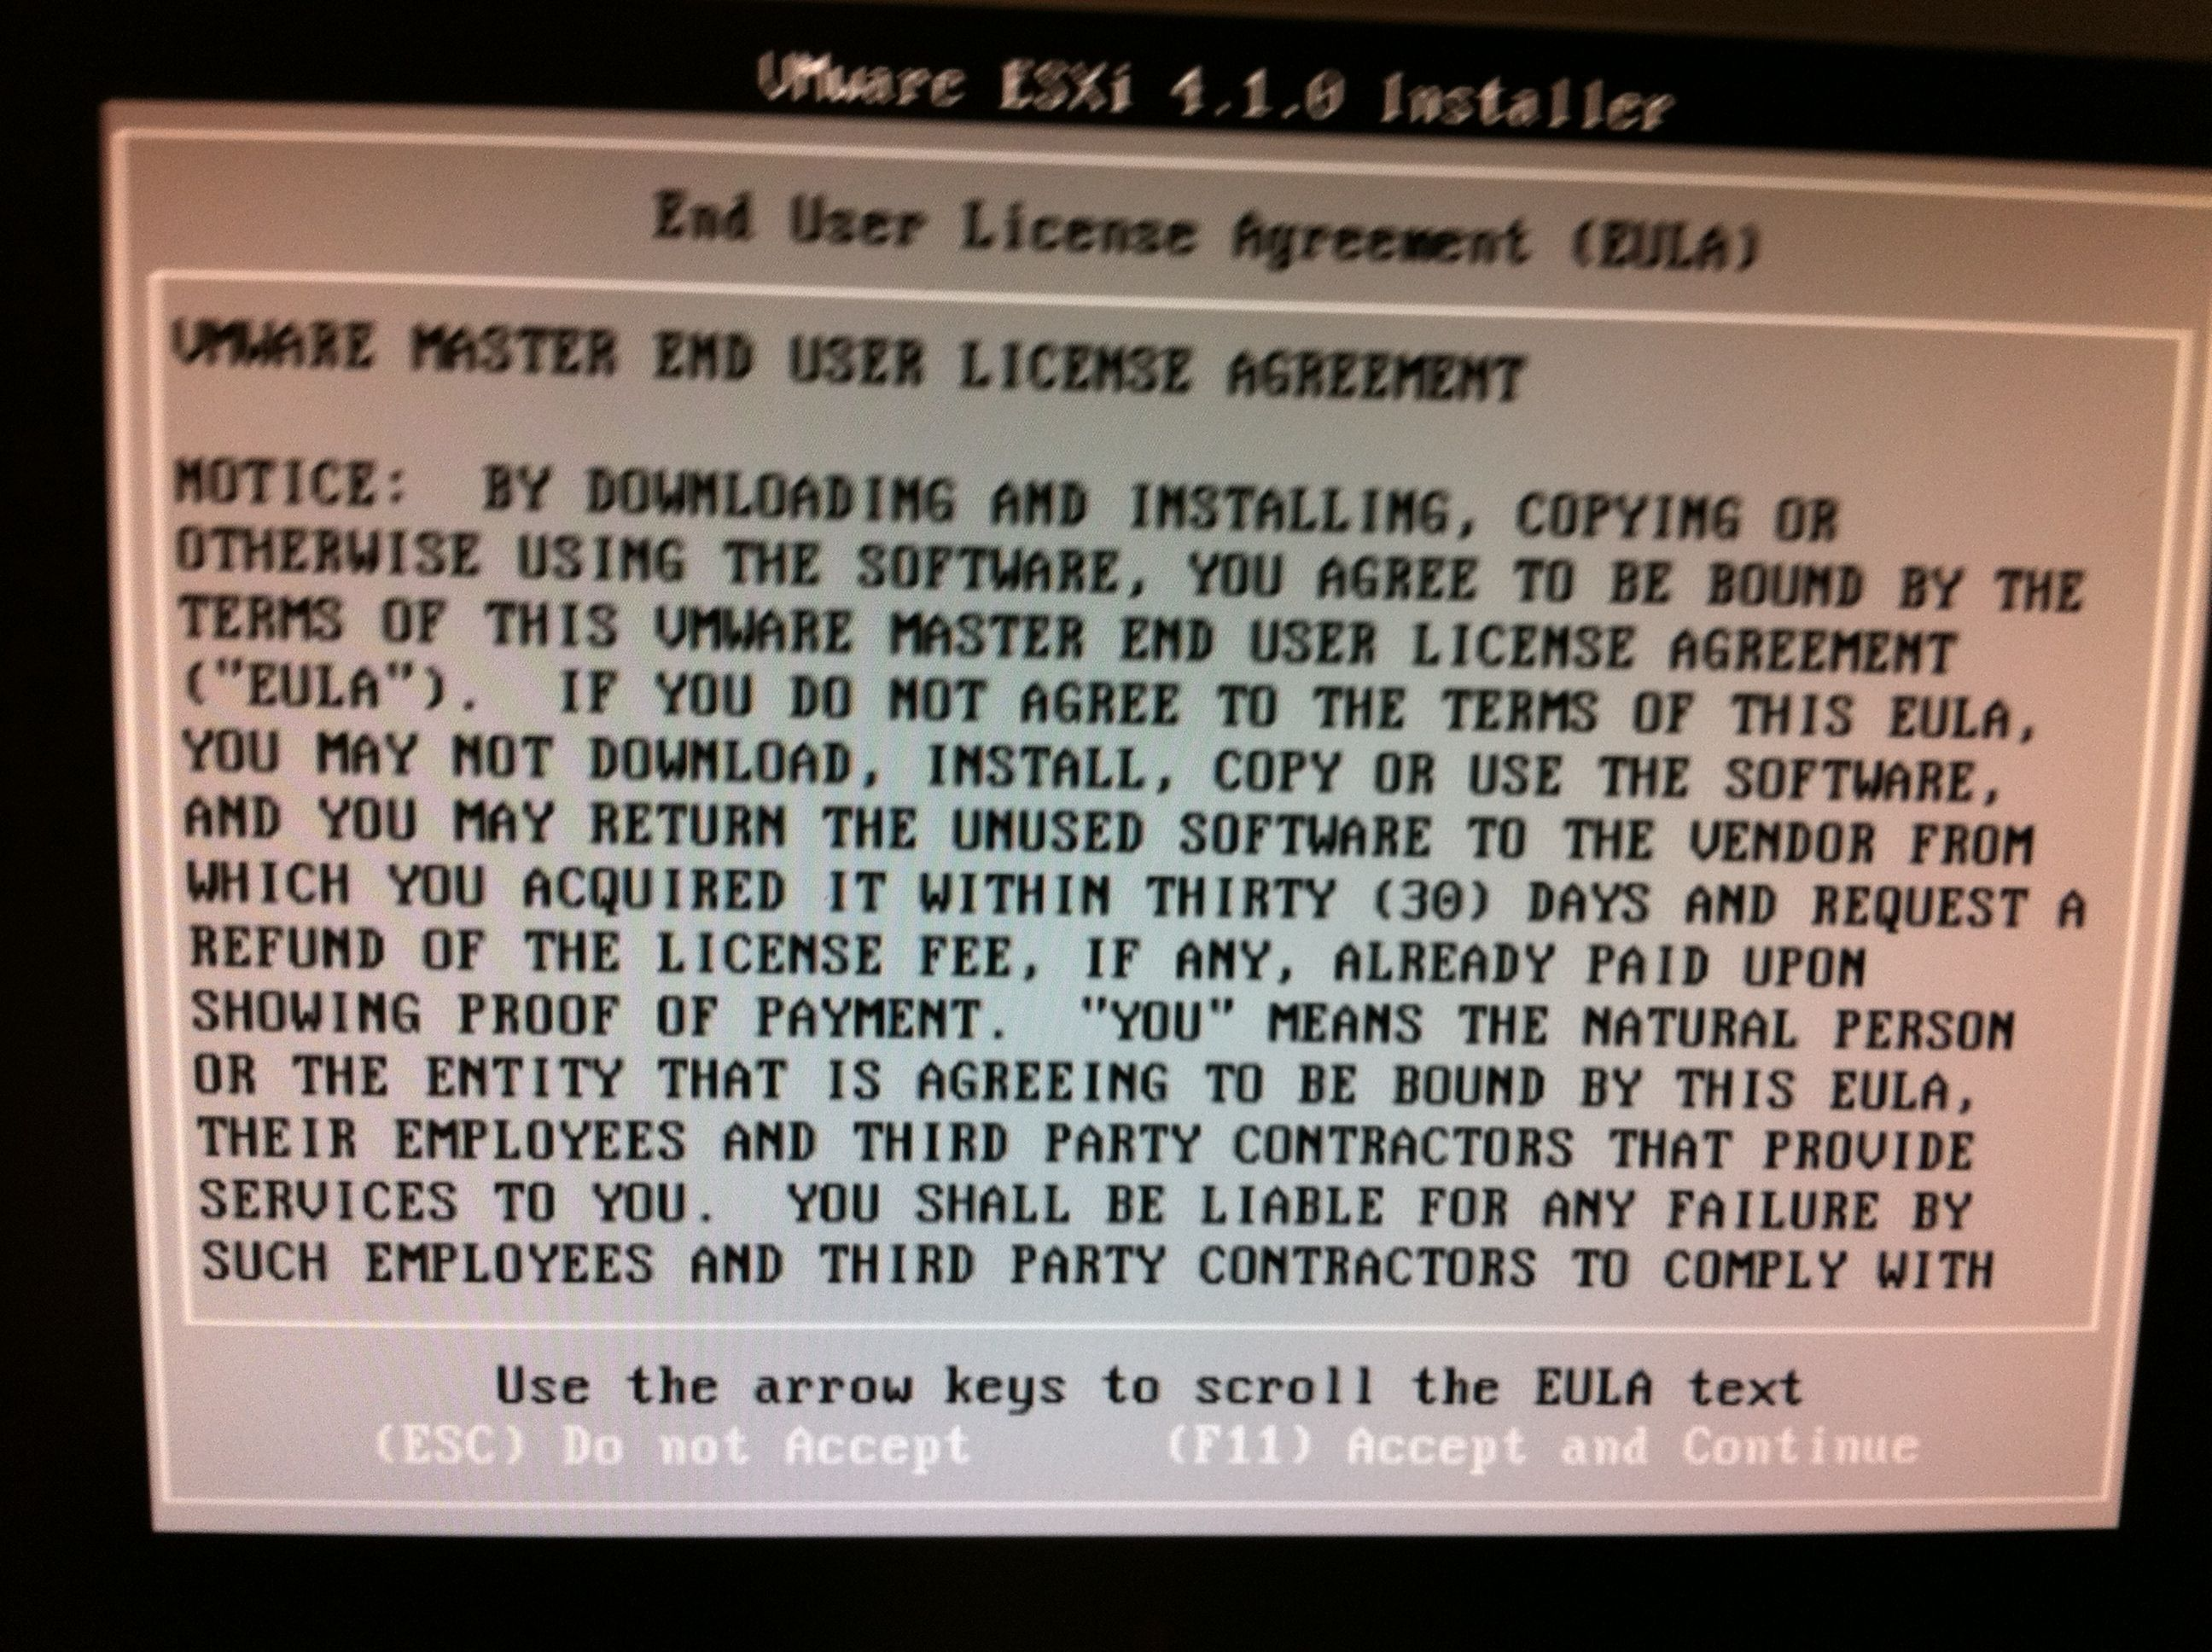
\includegraphics[width=0.5\textwidth]{./pic/esxi_3.jpg}
	\label{fig:kex_object_creation}
\end{figure}

\textbf{Step 4:}\\
In this step, we will need to choose the disk to install VMware ESXi. We choose the correct destination disk and press "Enter"
\begin{figure}[ht]
	\caption{VMware ESXi disk selection}
  	\centering
	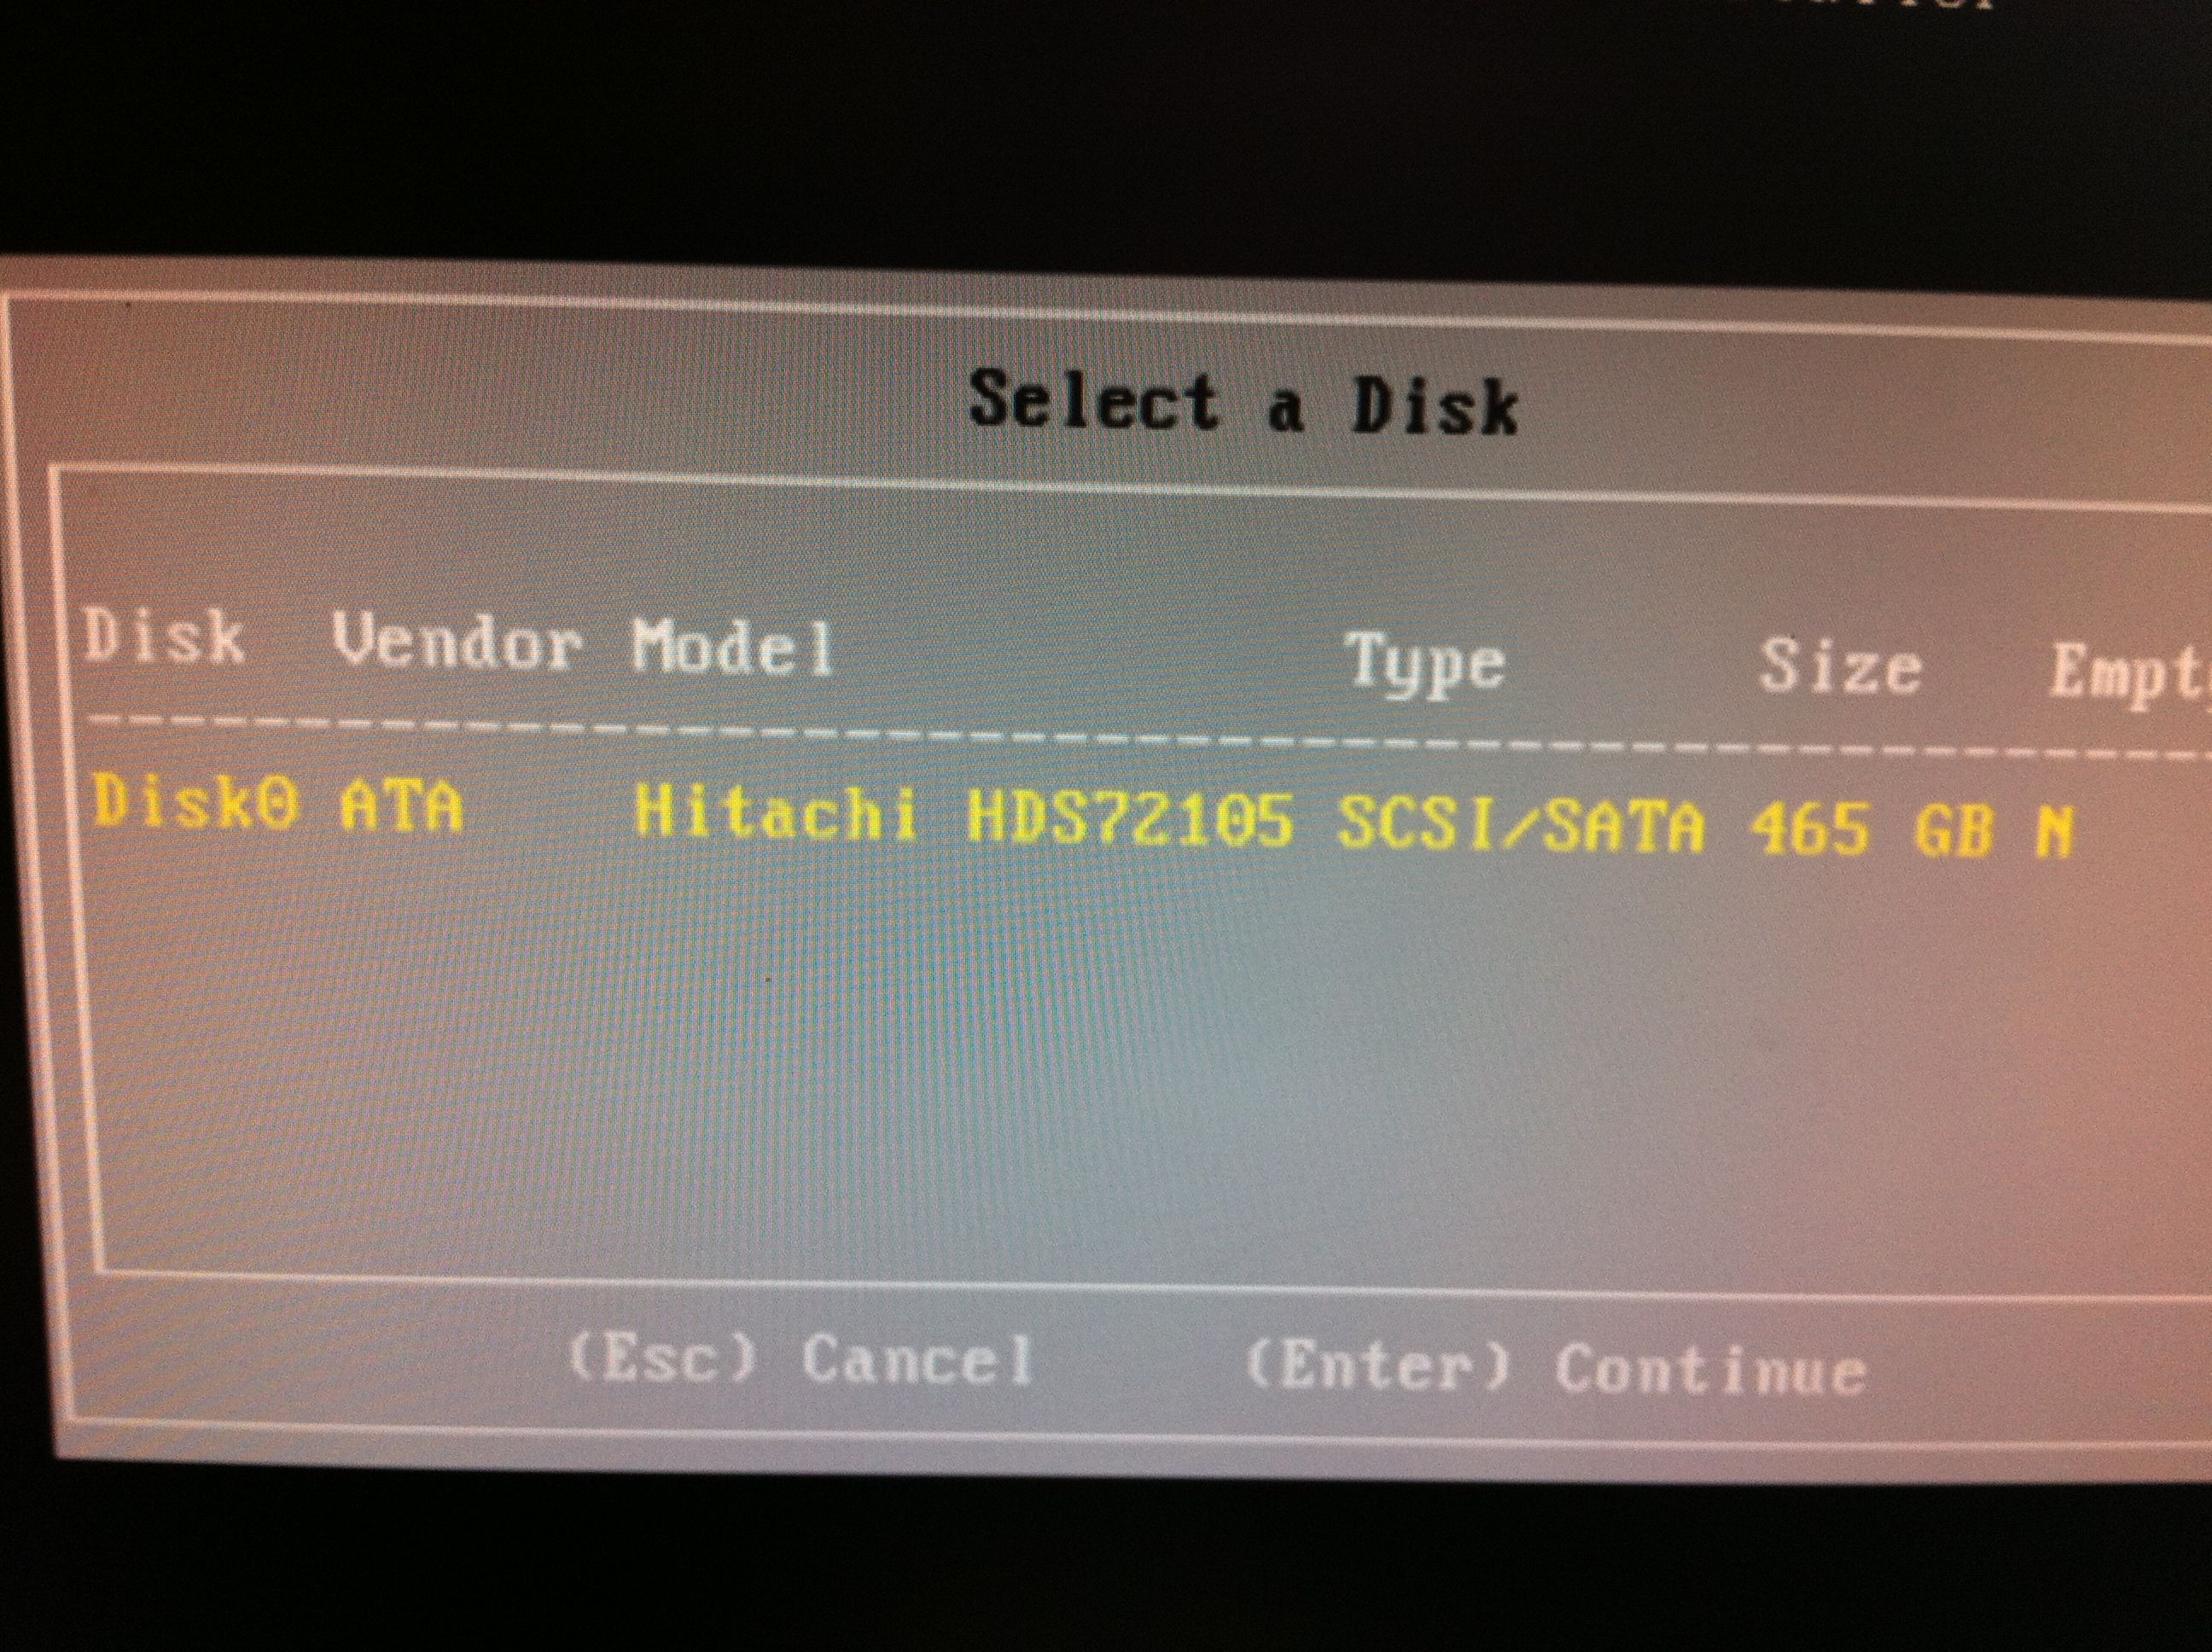
\includegraphics[width=0.5\textwidth]{./pic/esxi_4.jpg}
	\label{fig:kex_object_creation}
\end{figure}

\pagebreak
\textbf{Step 5: (optional)}\\
The installation program may ask if we want to erase the data containing on the destination disk. We will erase the data by pressing the "Enter" key. 
\begin{figure}[ht]
	\caption{VMware ESXi disk selection (confirmation)}
  	\centering
	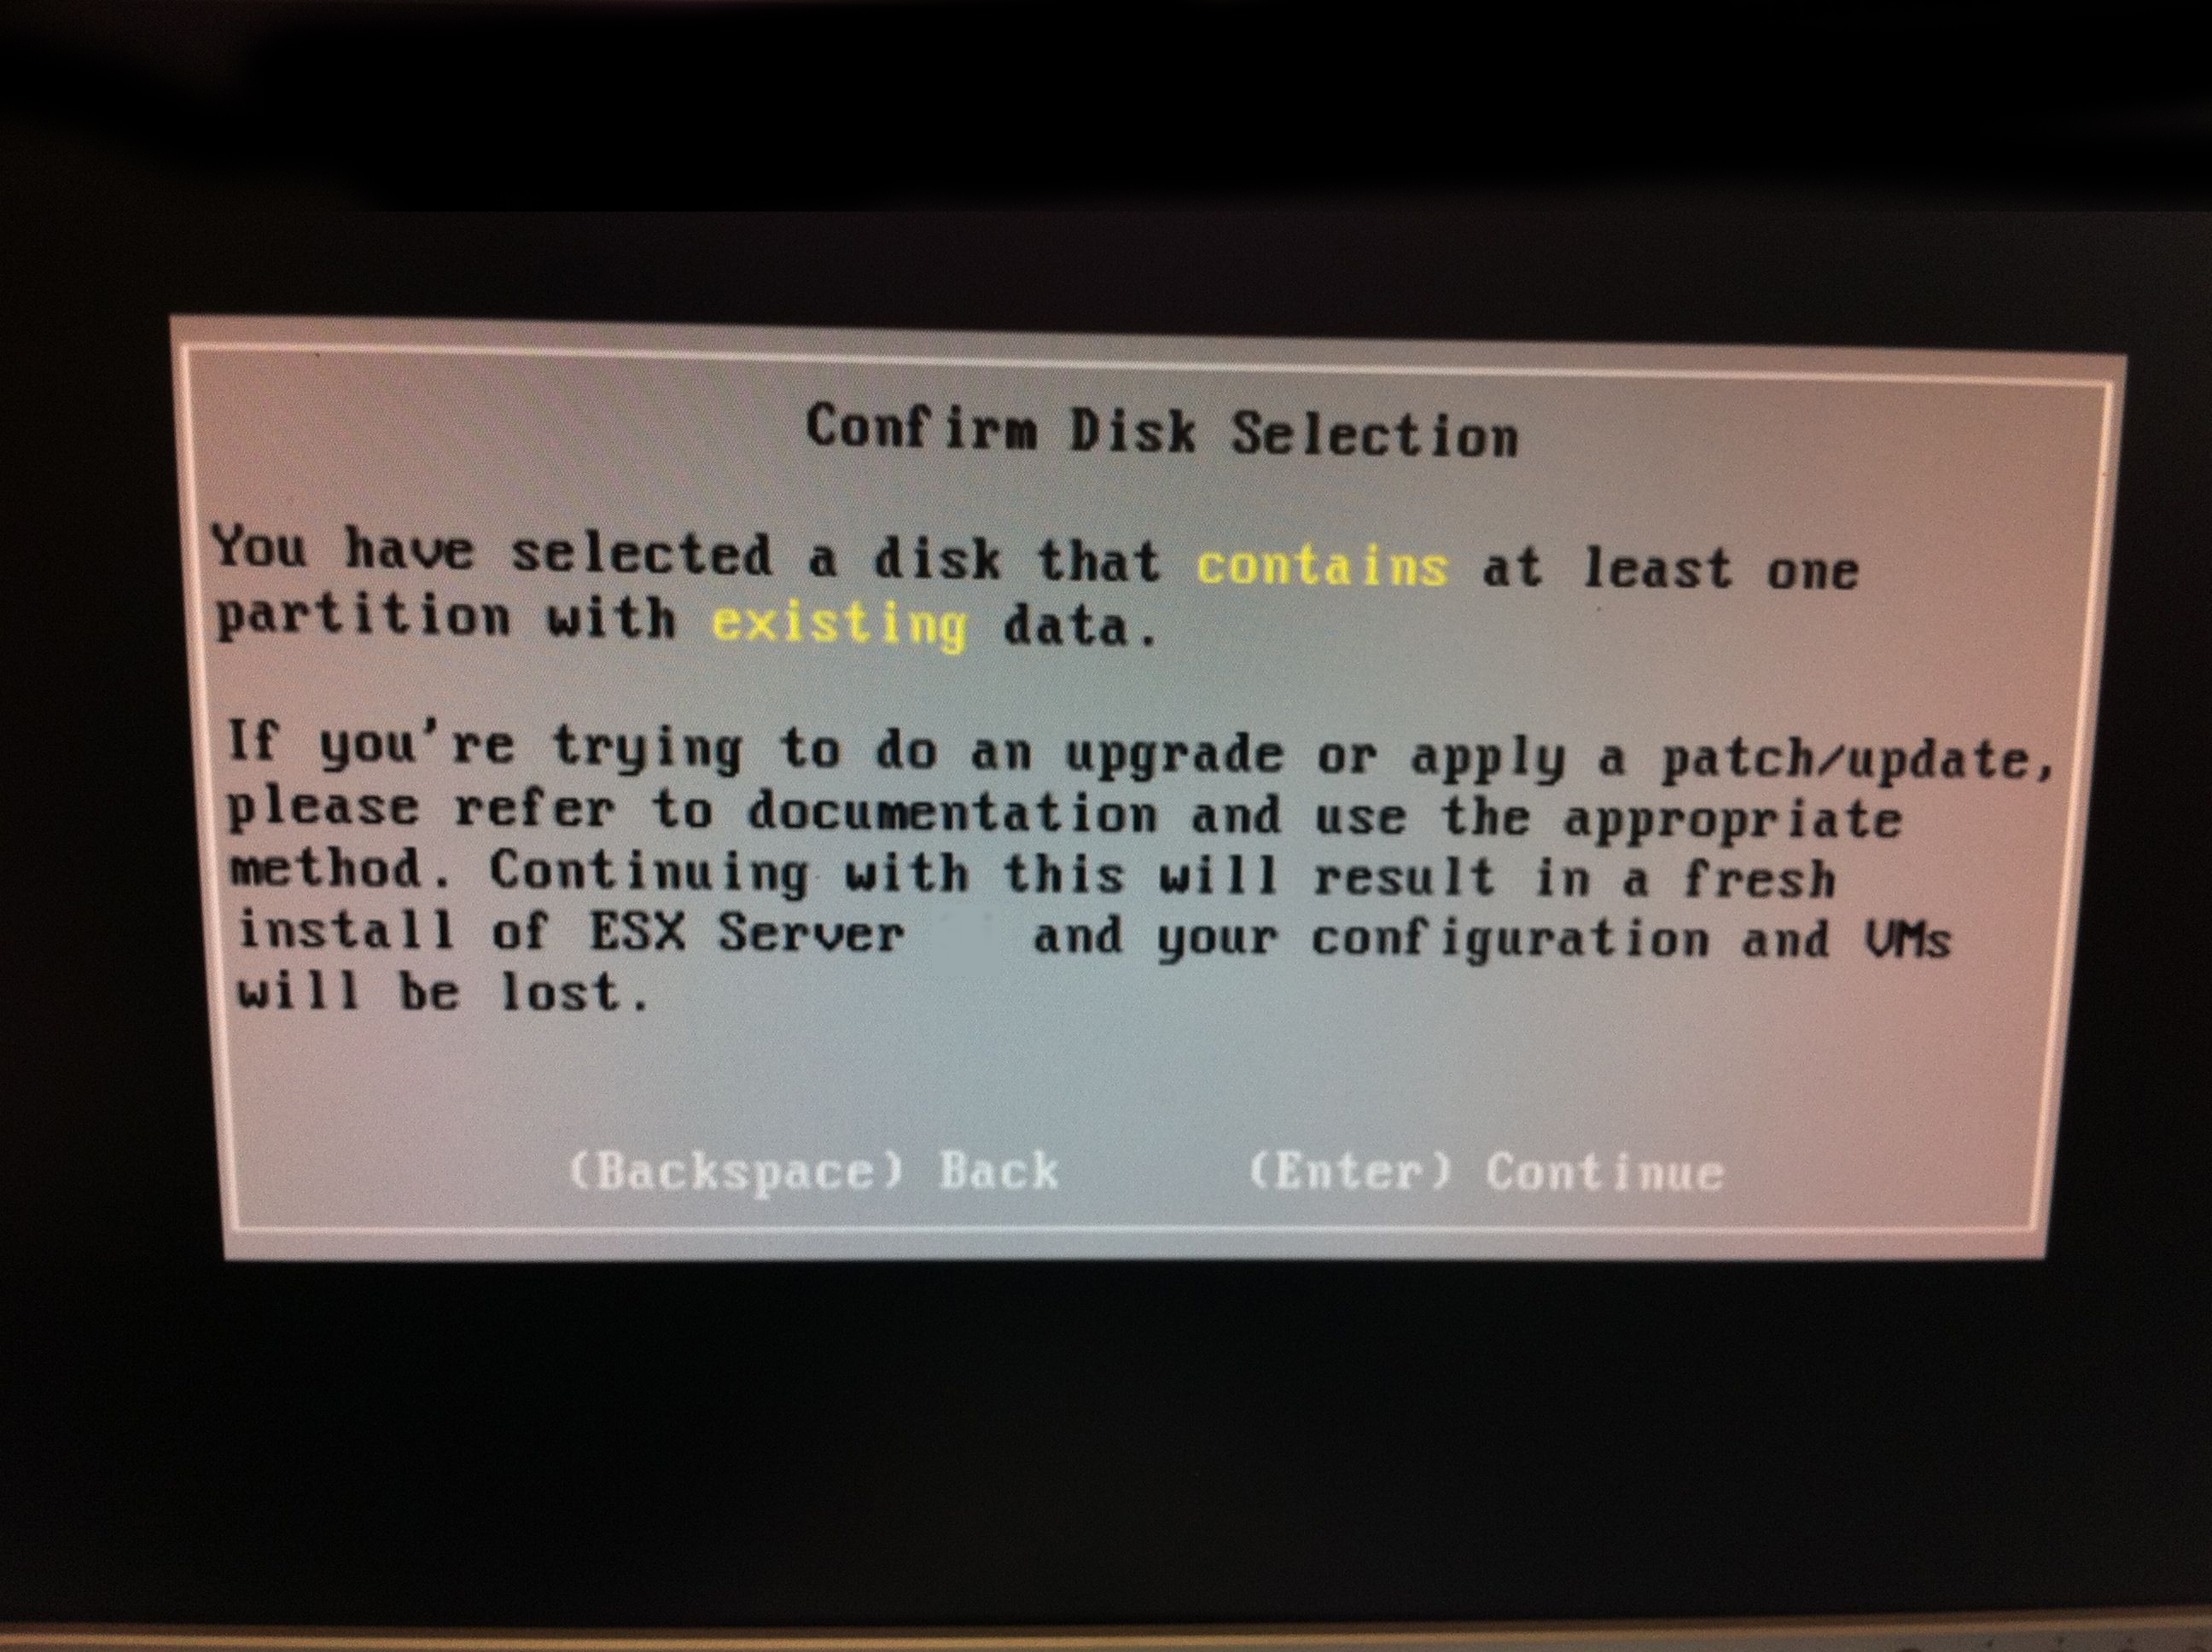
\includegraphics[width=0.5\textwidth]{./pic/esxi_5.jpg}
	\label{fig:kex_object_creation}
\end{figure}

\textbf{Step 6:}\\
We are ready to launch the installation of VMware ESXi on the computer. The installation program will ask us to confirm the installation by pressing the "F11" key. 
\begin{figure}[ht]
	\caption{VMware ESXi Installation confirmation}
  	\centering
	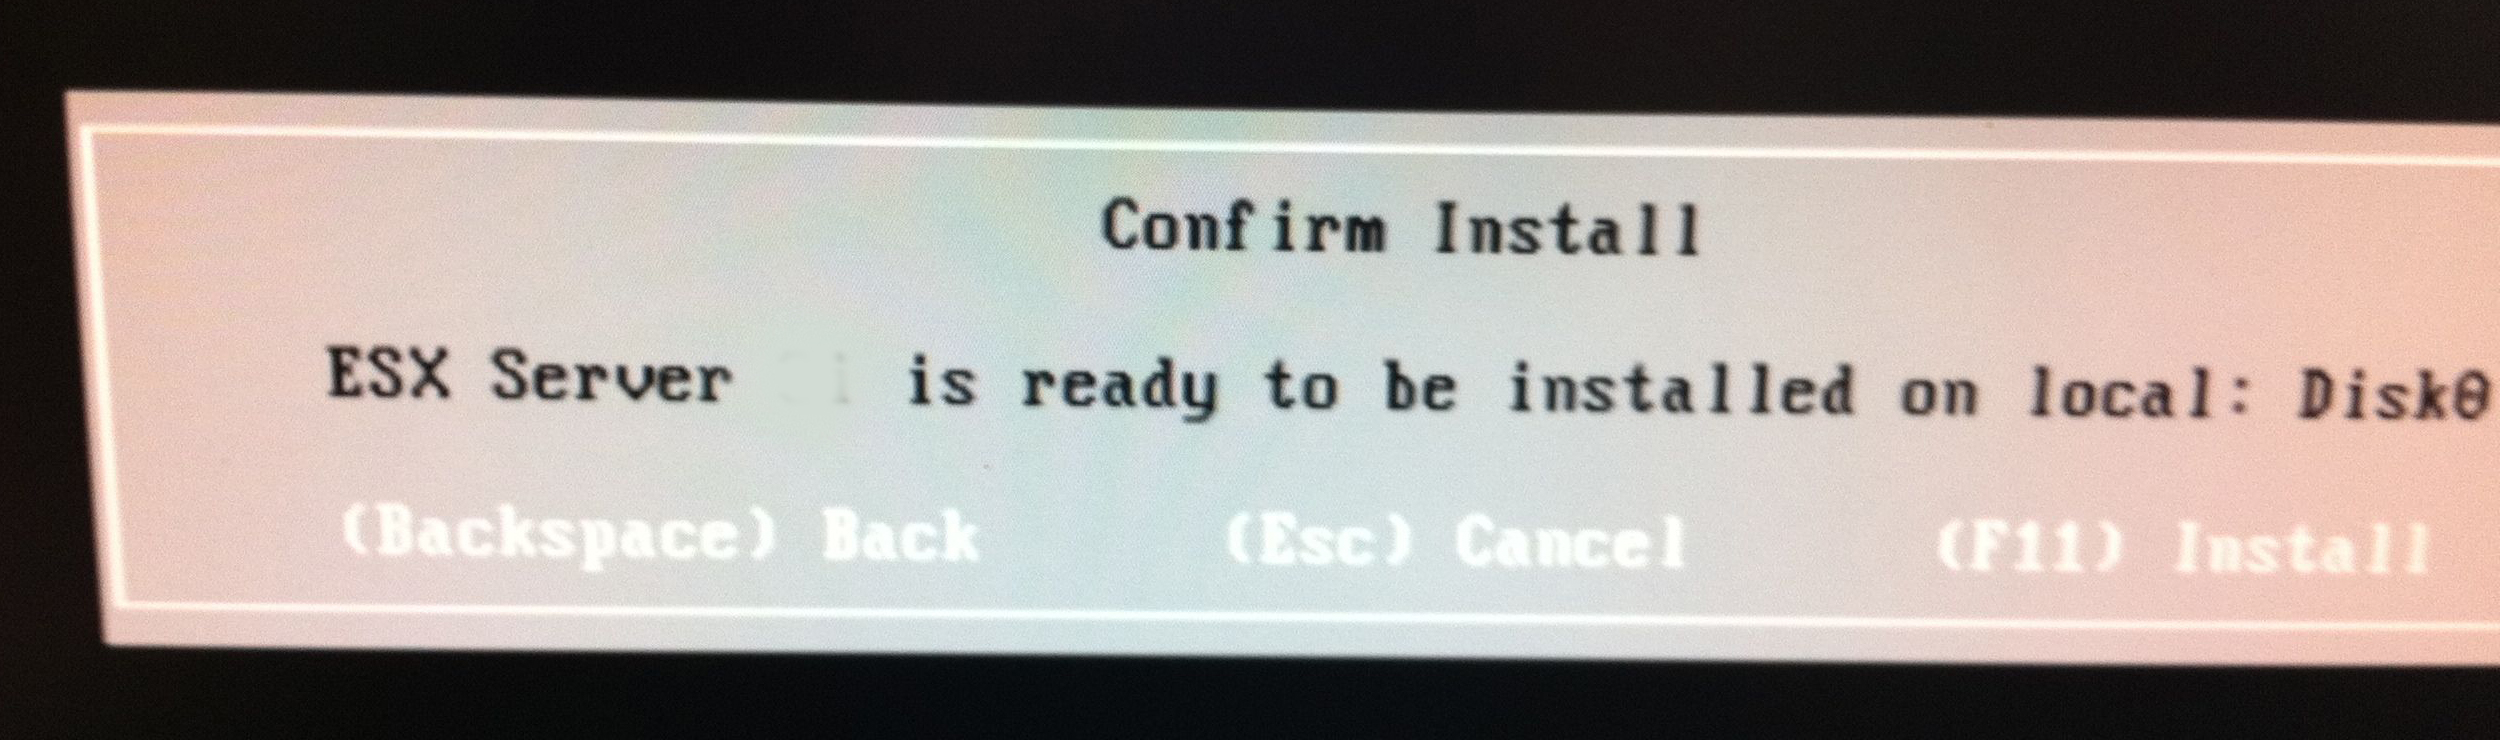
\includegraphics[width=0.7\textwidth]{./pic/esxi_6.jpg}
	\label{fig:kex_object_creation}
\end{figure}


\pagebreak
\textbf{ESXi configuration}
As the ESXi platform will act as a server, we will need to configure the network parameter and the credentials. When the ESXi system is started, the first screen looks like Firgure \ref{fig:esxi_first_screen}. To be able to change any system parameters, we need to press the "F2" key.\s

\begin{figure}[ht]
	\caption{VMware ESXi Startup screen}
  	\centering
	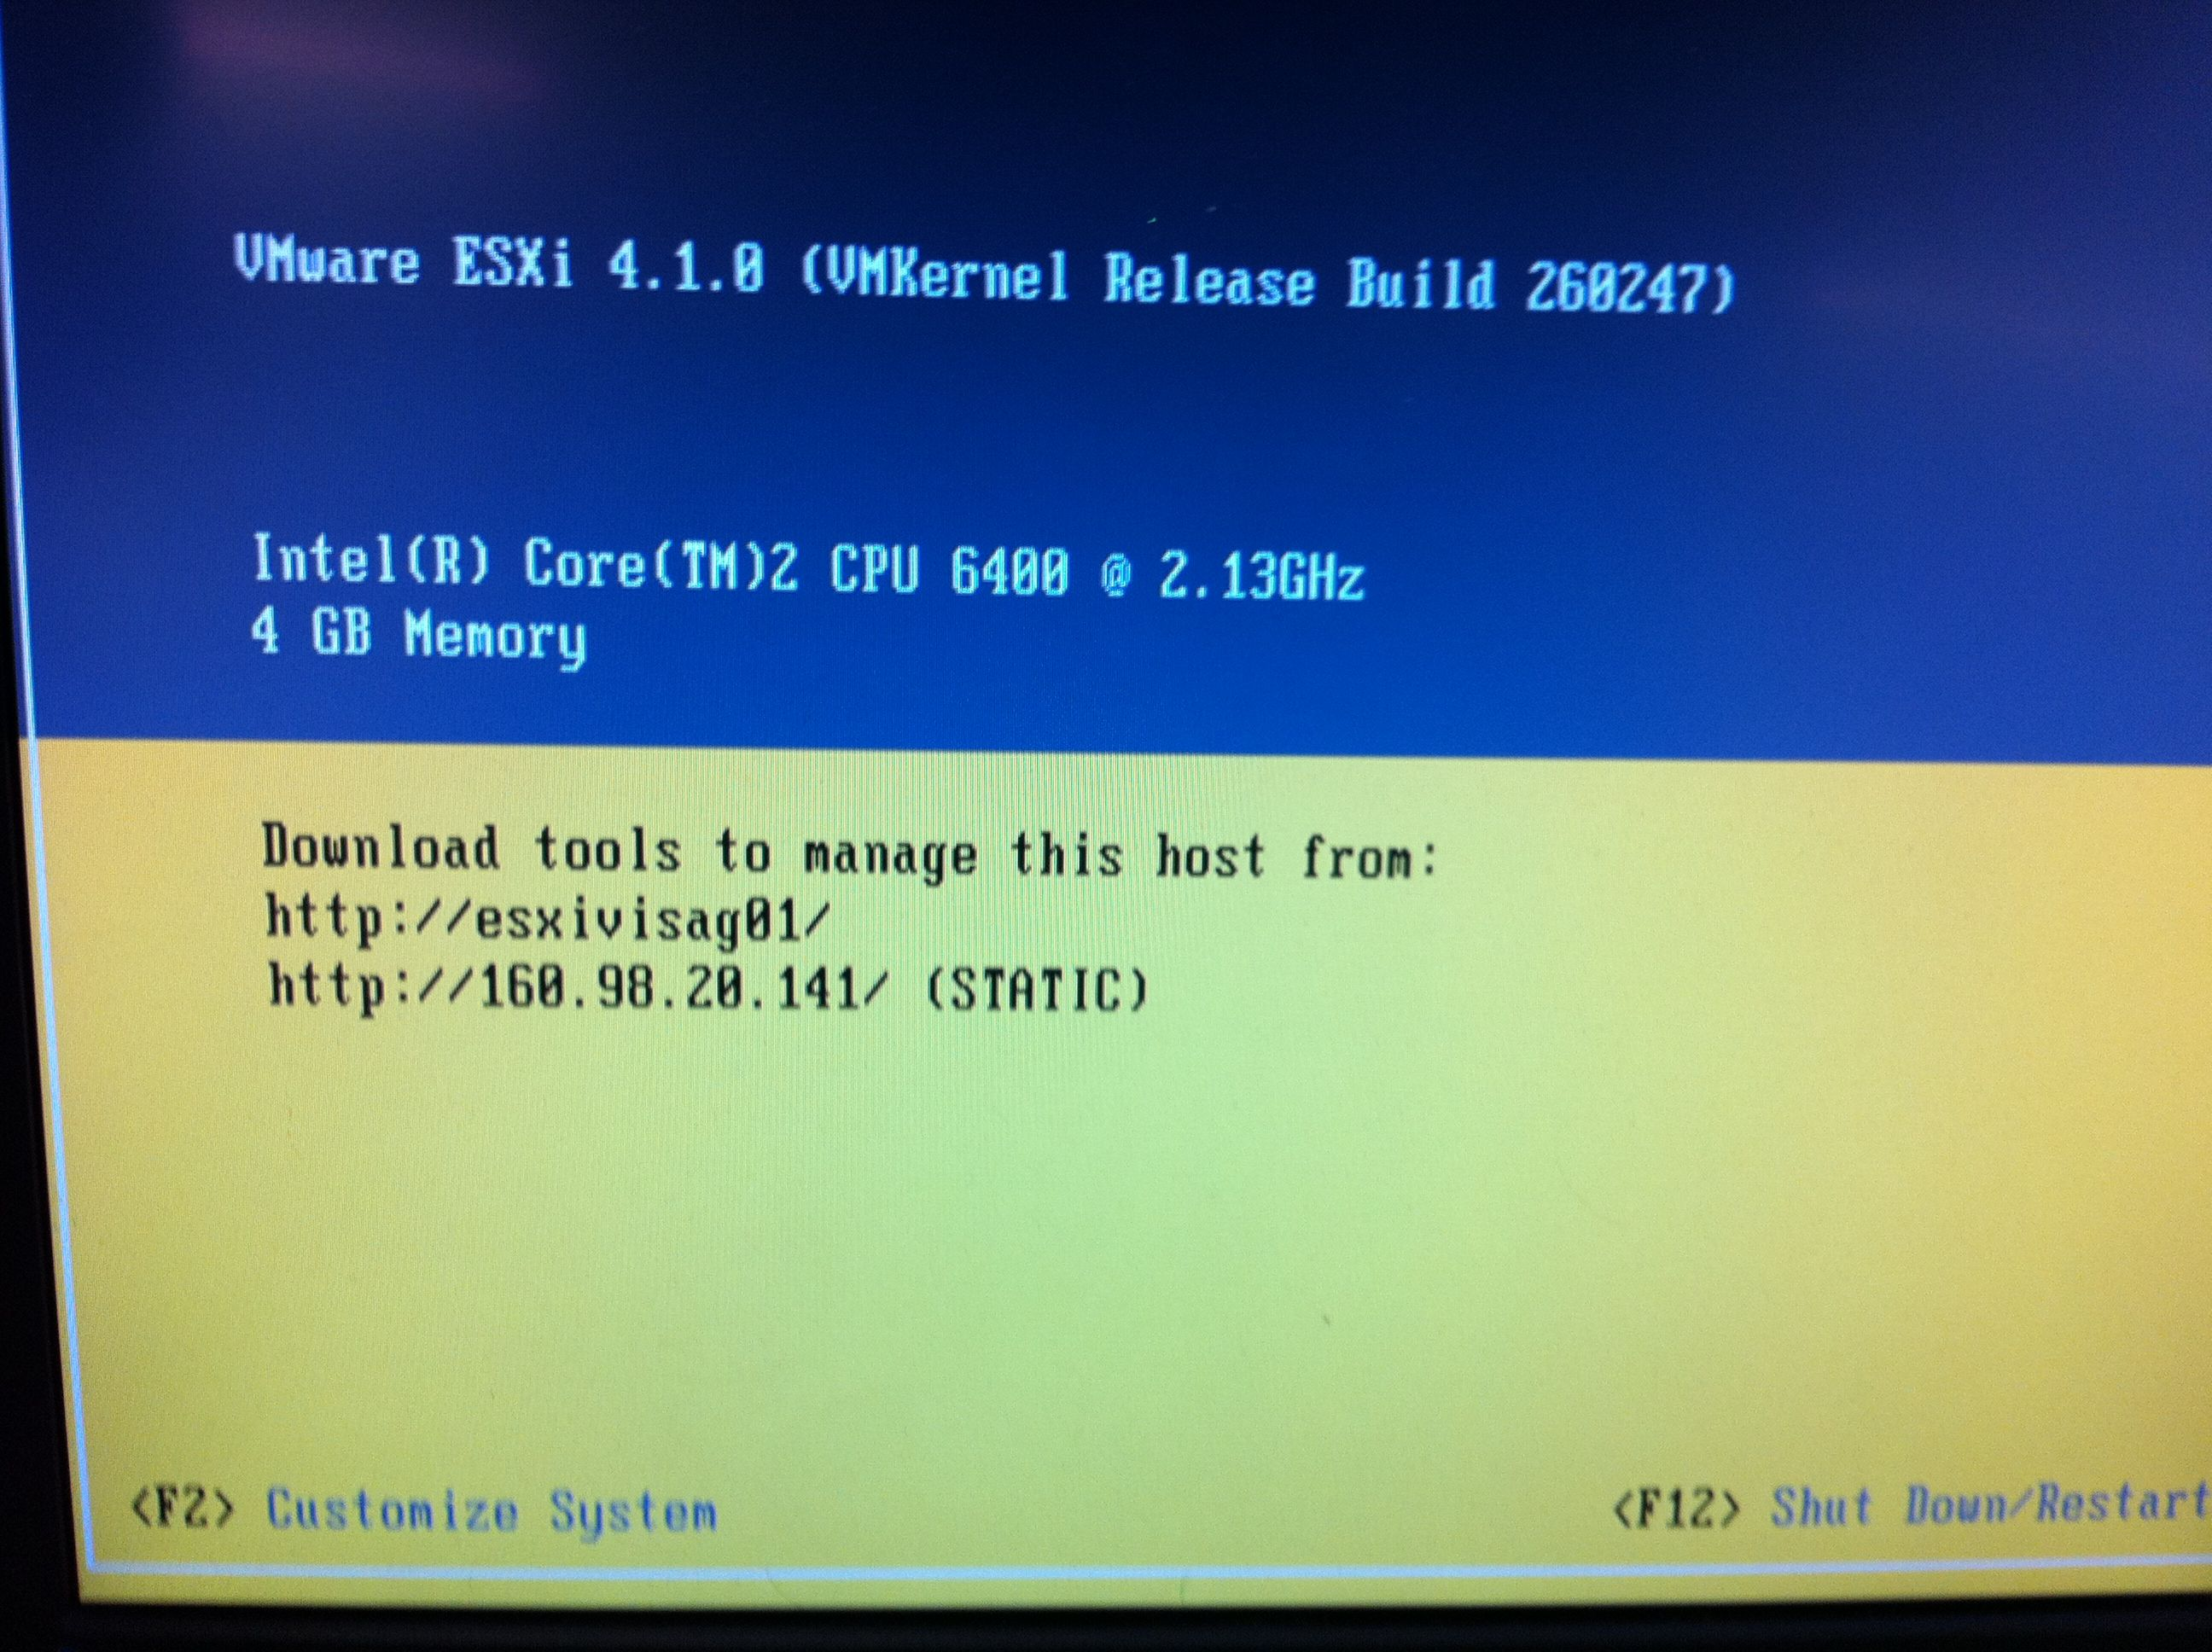
\includegraphics[width=0.5\textwidth]{./pic/esxi_7.jpg}
	\label{fig:esxi_first_screen}
\end{figure}

If a password is already set up, a login screen will appear like in Figure \ref{fig:esxi_login}. Just enter the password and press the "Enter key".
\begin{figure}[ht]
	\caption{VMware ESXi Login screen}
  	\centering
	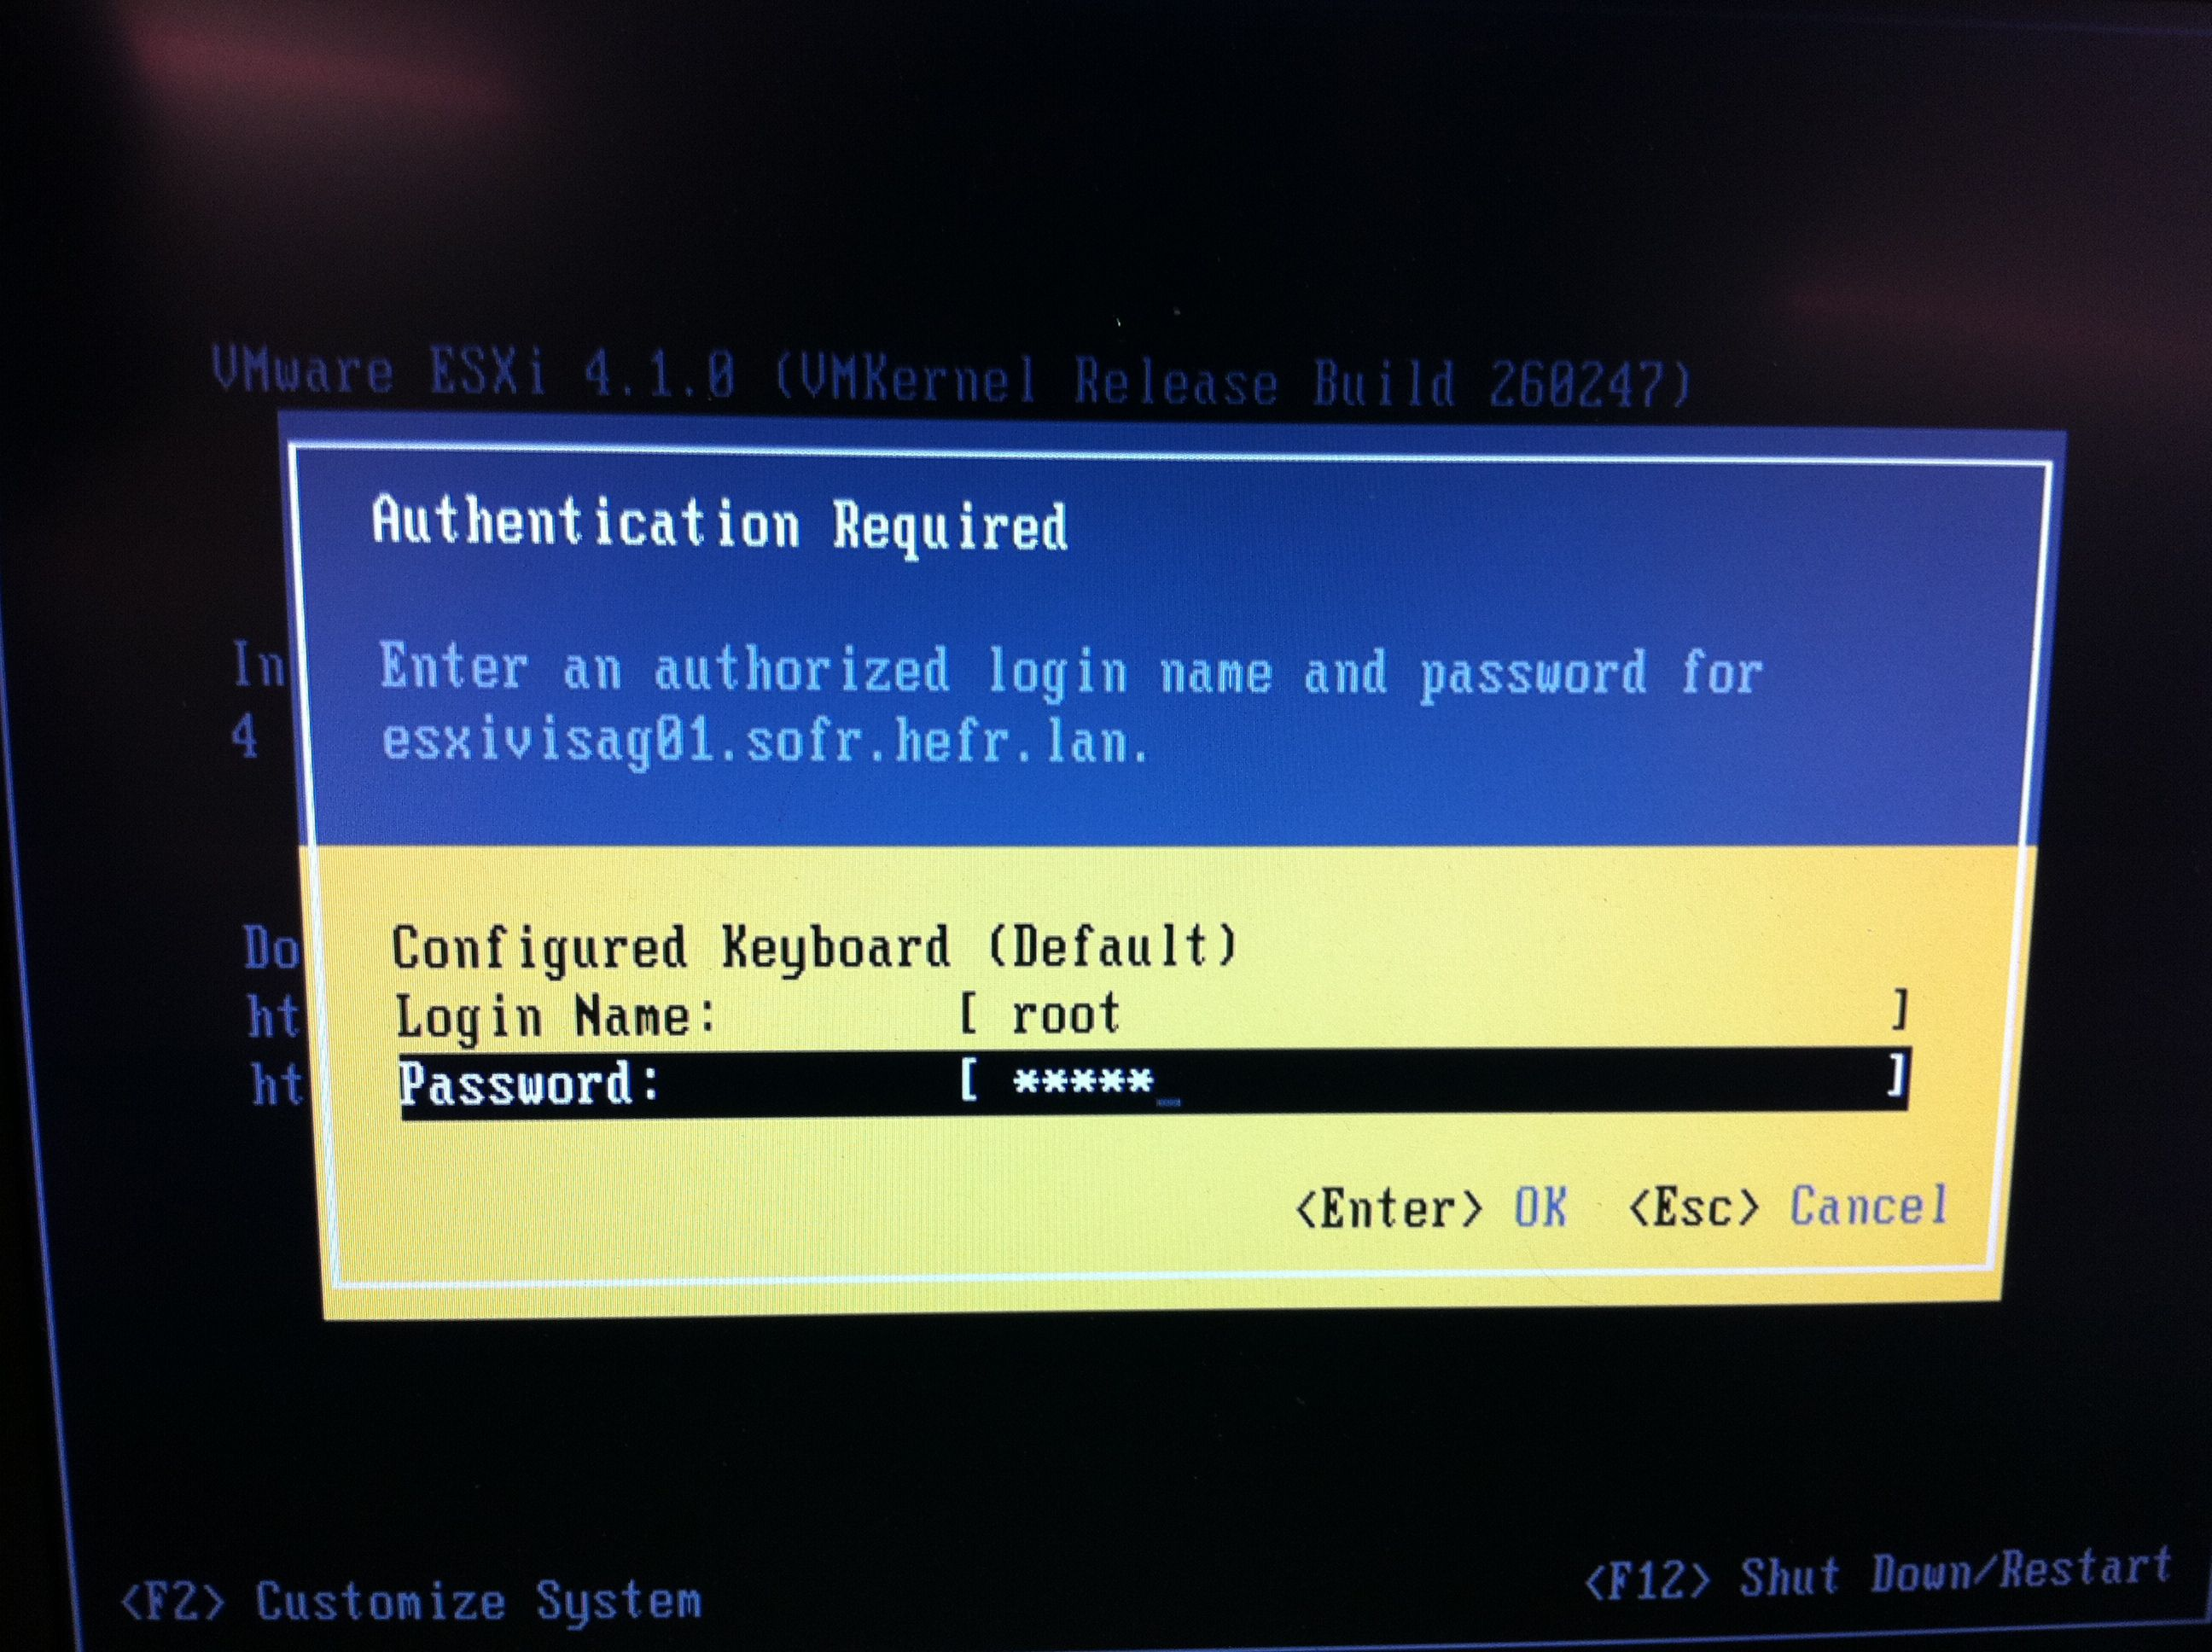
\includegraphics[width=0.5\textwidth]{./pic/esxi_8.jpg}
	\label{fig:esxi_login}
\end{figure}

\pagebreak
\textbf{Network configuration}\\
The ESXi platform needs a static IP address to work well with POP-C++ Virtual. Once logged into the ESXi system, we can modify the IP parameter in the "Configure Management Network" section (see Figure \ref{fig:esxi_sysconf}).

\begin{figure}[ht]
	\caption{VMware ESXi System configuration}
  	\centering
	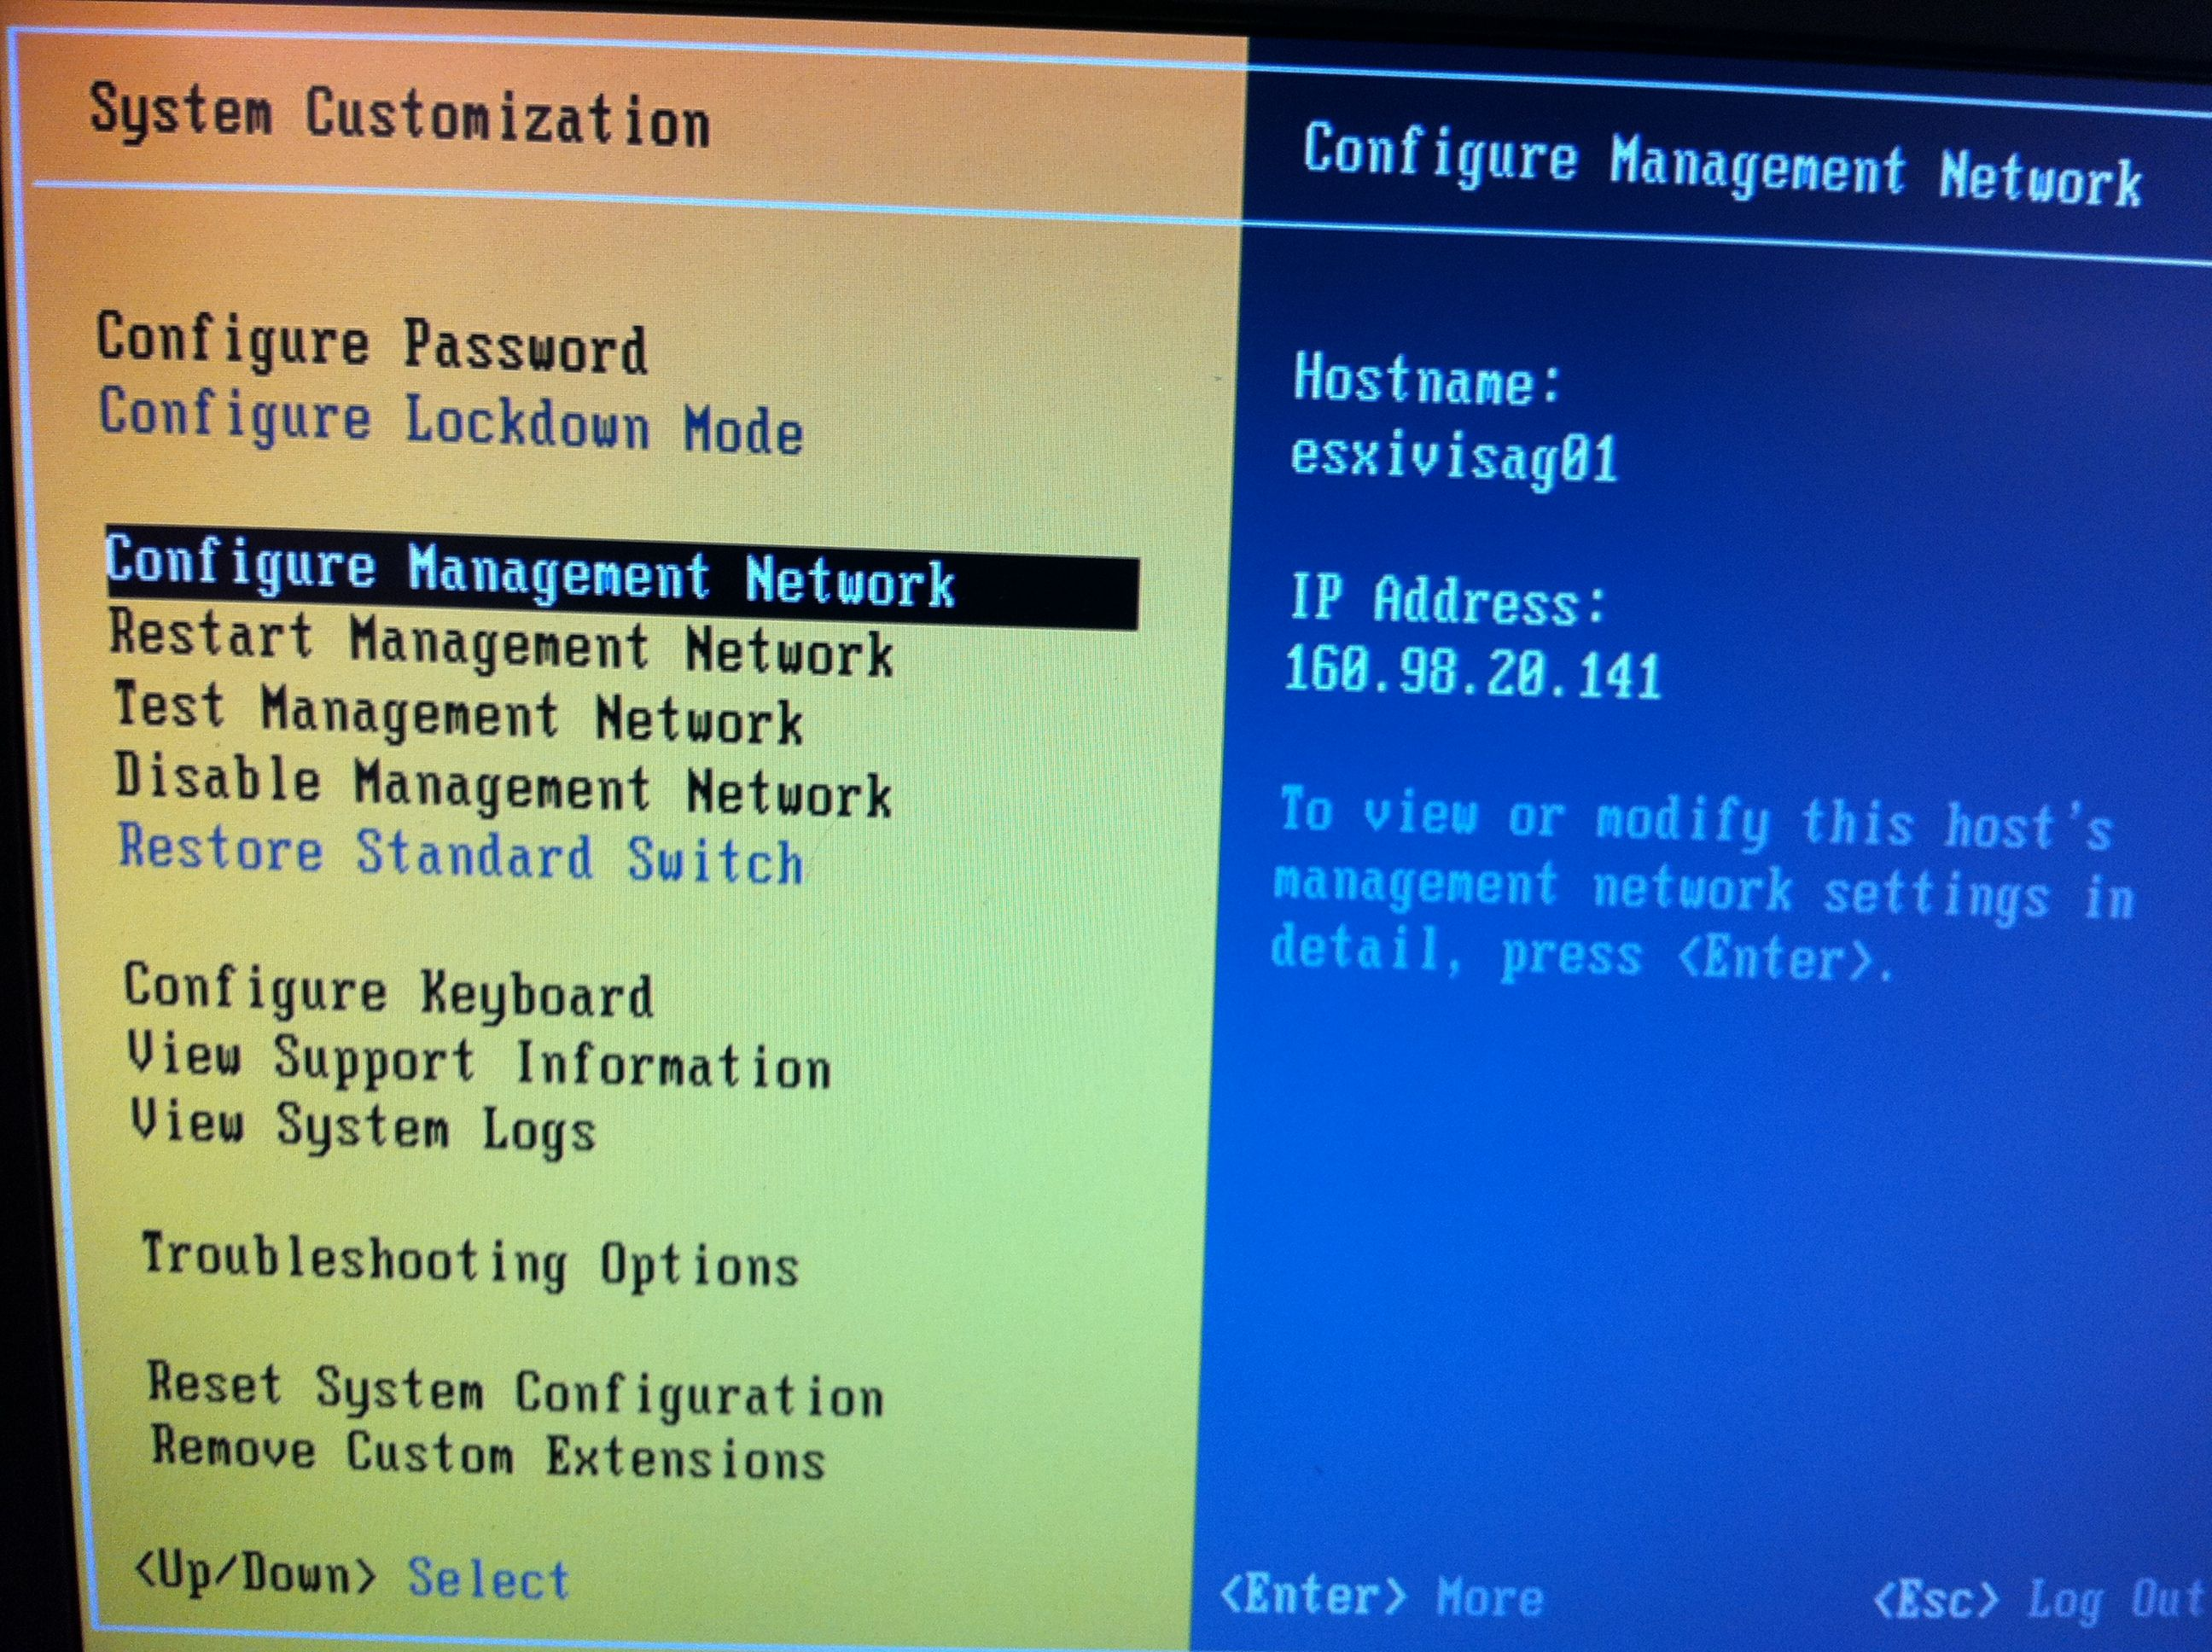
\includegraphics[width=0.5\textwidth]{./pic/esxi_9.jpg}
	\label{fig:esxi_sysconf}
\end{figure}

In the "Configure Management Network" section, we can select the "IP Configuration" subsection to modify the IPv4 parameter (see Figure \ref{fig:esxi_sysconf_ip}).

\begin{figure}[ht]
	\caption{VMware ESXi Network Management Configuration}
  	\centering
	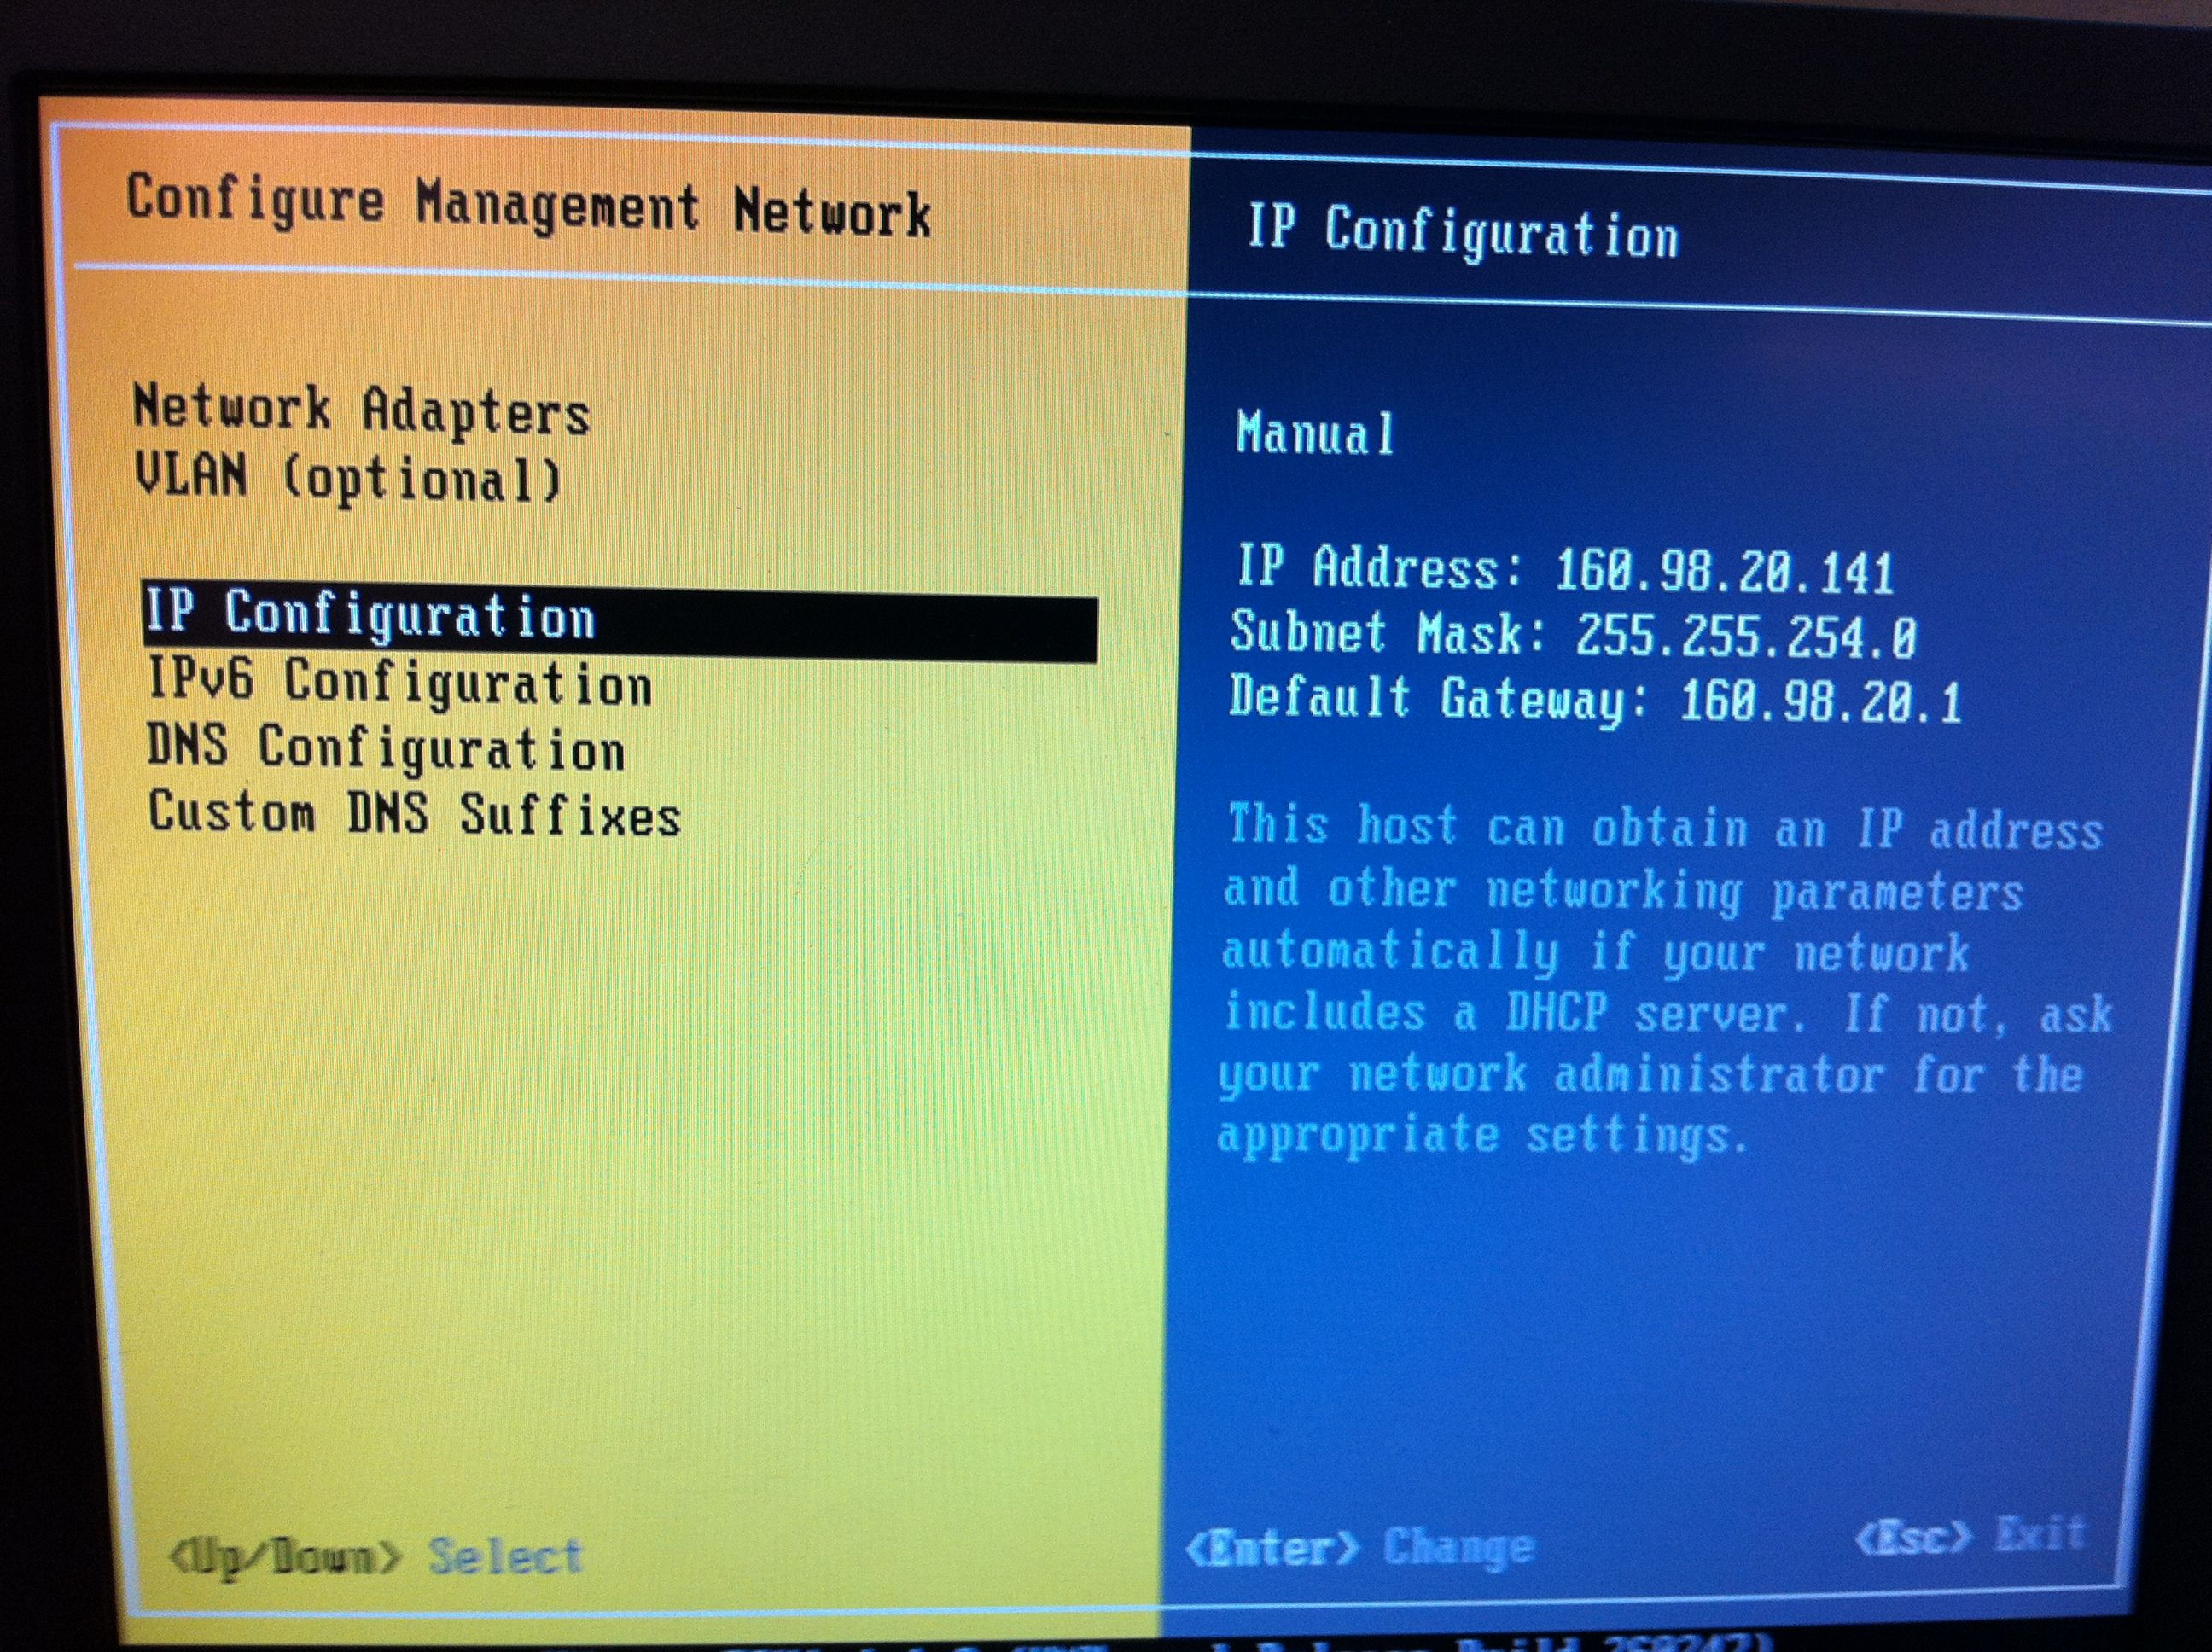
\includegraphics[width=0.5\textwidth]{./pic/esxi_10.jpg}
	\label{fig:esxi_sysconf_ip}
\end{figure}

\pagebreak
Once in the IP Configuration subsection, we can select "Set static IP address and network configuration" and fill the fields below (see Figure \ref{fig:esxi_sysconf_ipv4}). When the information are set, we can save them by pressing the "Enter" key. 

\begin{figure}[ht]
	\caption{VMware ESXi IPv4 Configuration}
  	\centering
	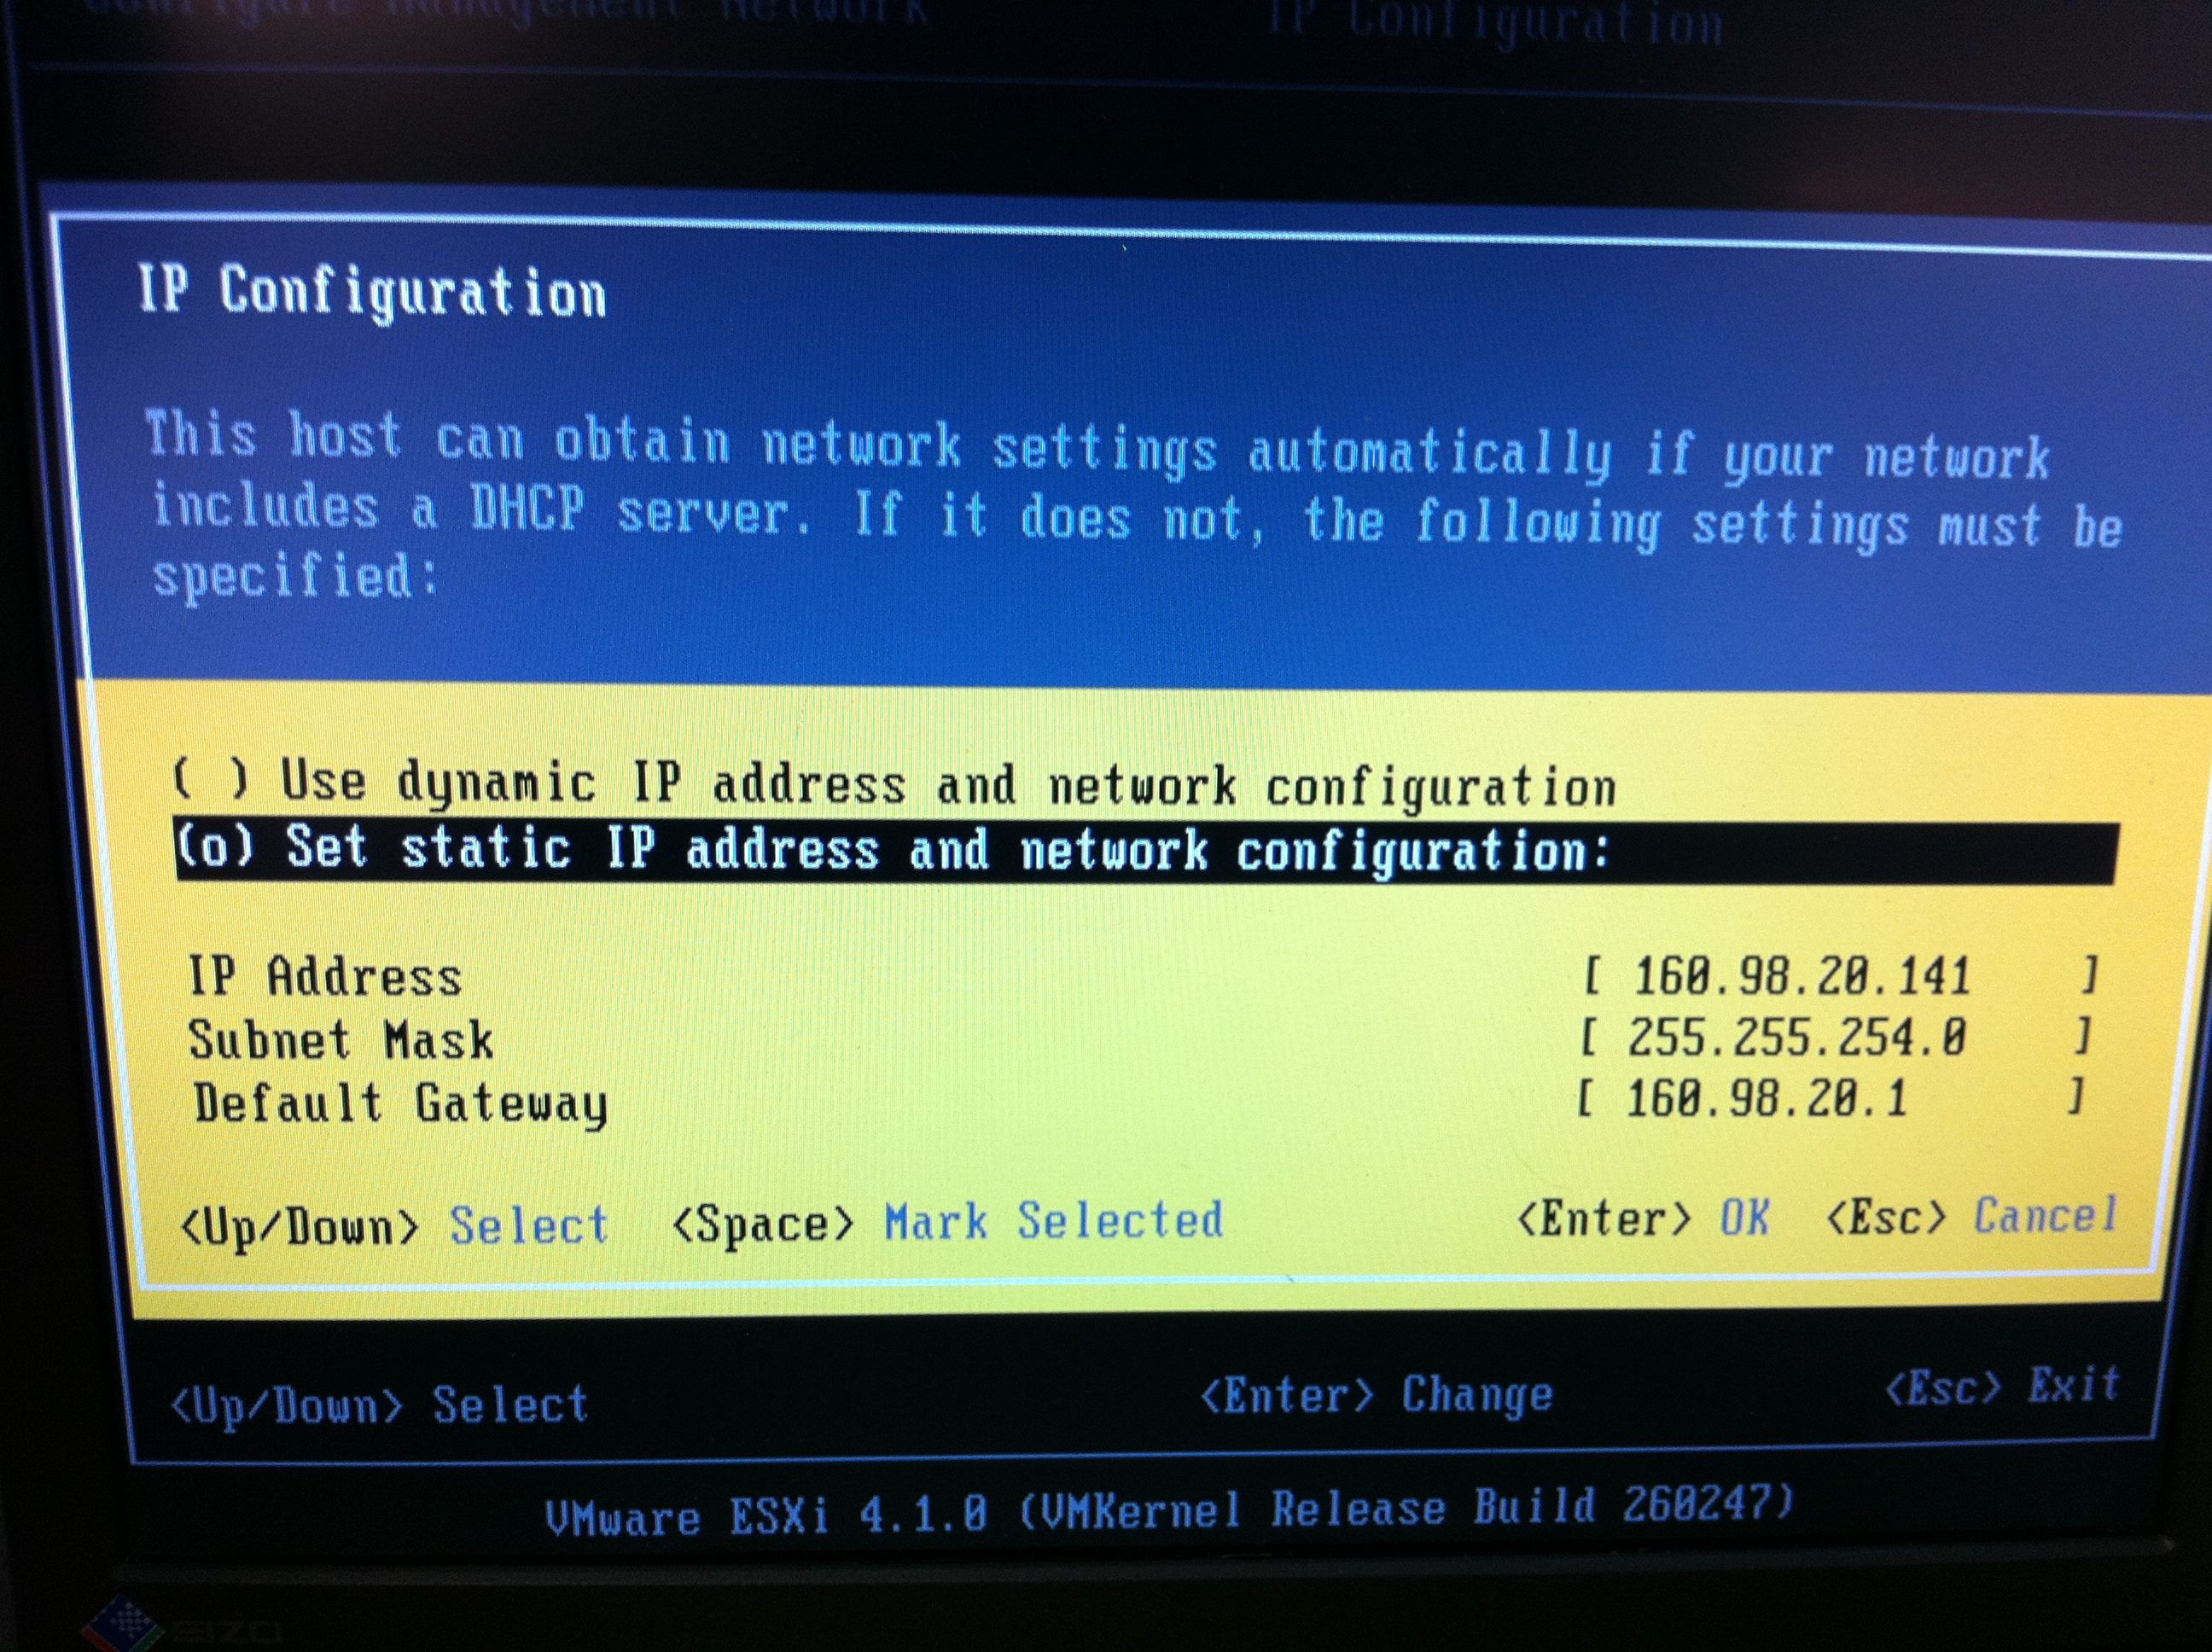
\includegraphics[width=0.5\textwidth]{./pic/esxi_11.jpg}
	\label{fig:esxi_sysconf_ipv4}
\end{figure}


After setting the IPv4 parameters, we need to set up the DNS parameter. In the "Configure Management Network", we will choose "DNS configuration" instead of "IP configuration" (see Figure \ref{fig:esxi_sysconf_ip}). Like in Figure \ref{fig:esxi_sysconf_dns}, we select "Use the following DNS server addresses and hostname" and fill the fields. \s

\textit{NOTE:} This step is not mandatory if you have a unique DNS name attributed by IP address. But your ESXi host must be reachable by its DNS hostname. 
\begin{figure}[ht]
	\caption{VMware ESXi System configuration}
  	\centering
	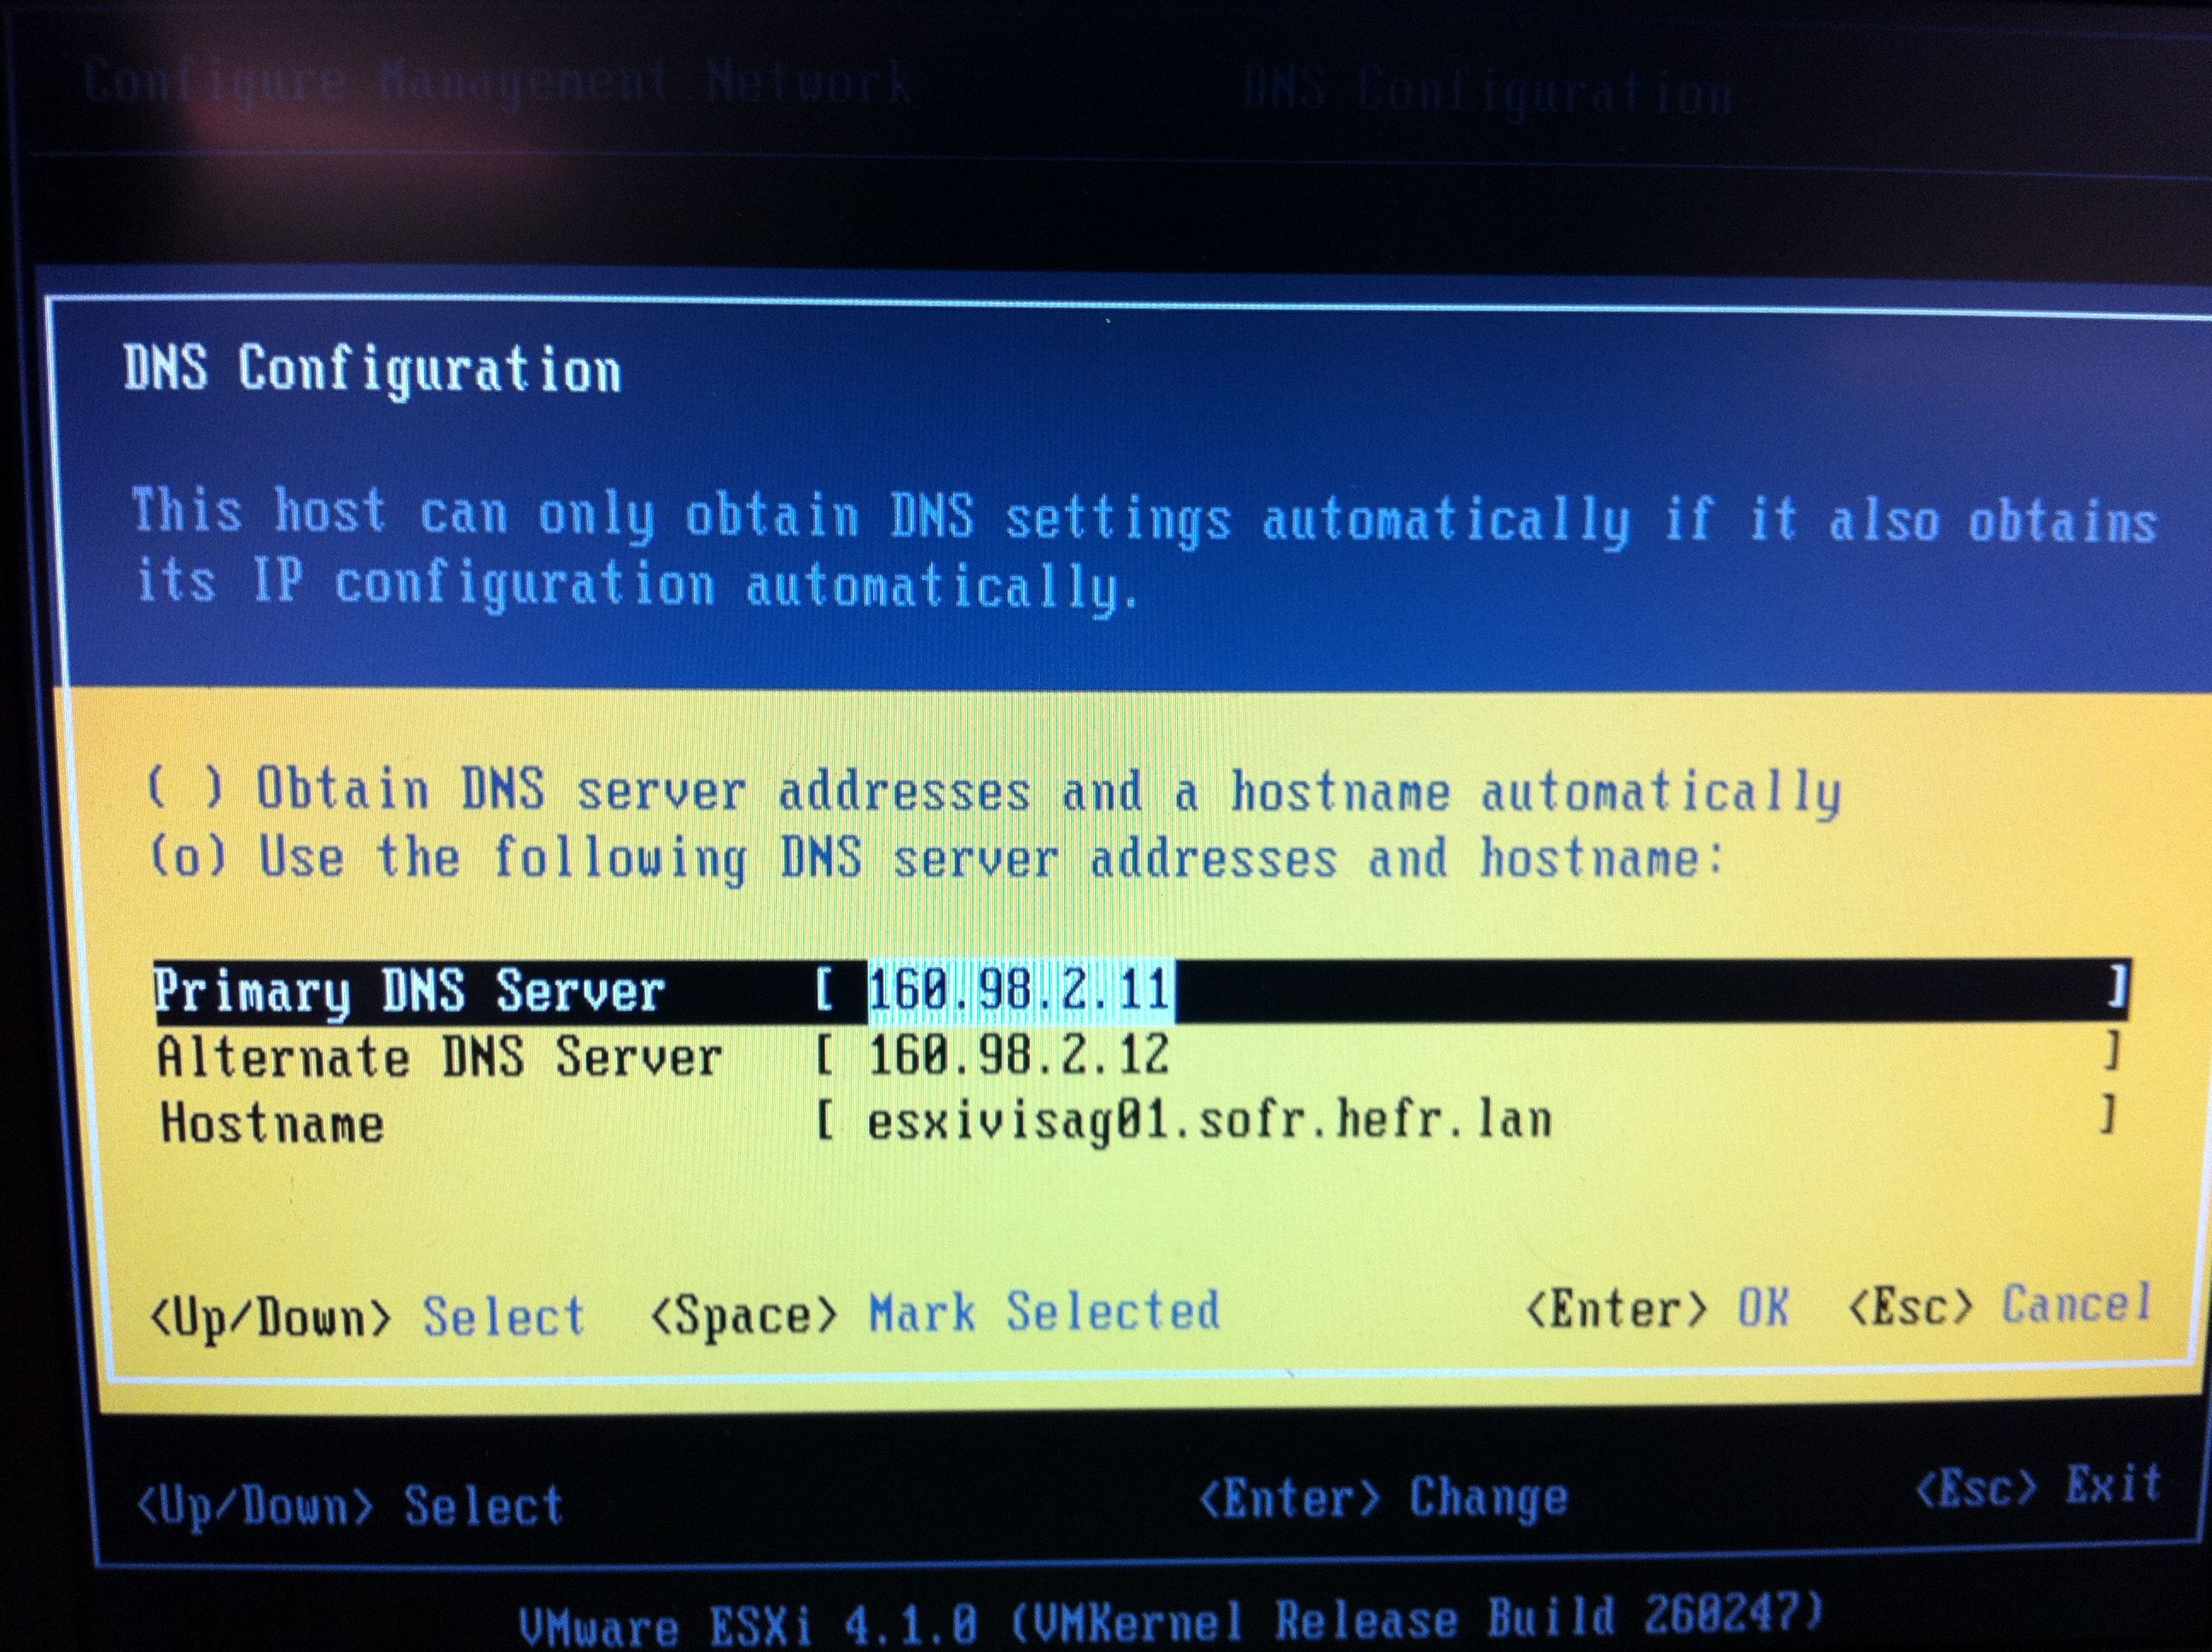
\includegraphics[width=0.5\textwidth]{./pic/esxi_12.jpg}
	\label{fig:esxi_sysconf_dns}
\end{figure}

\pagebreak

\textbf{Password configuration}\\
To set or change the administrator password, we will choose "Configure Password" in the ESXi System Configuration (see Figure \ref{fig:esxi_sysconf}). A screen will be prompted (Figure \ref{fig:esxi_sysconf_pass}) and we just need to fill it. 
\begin{figure}[ht]
	\caption{VMware ESXi System configuration}
  	\centering
	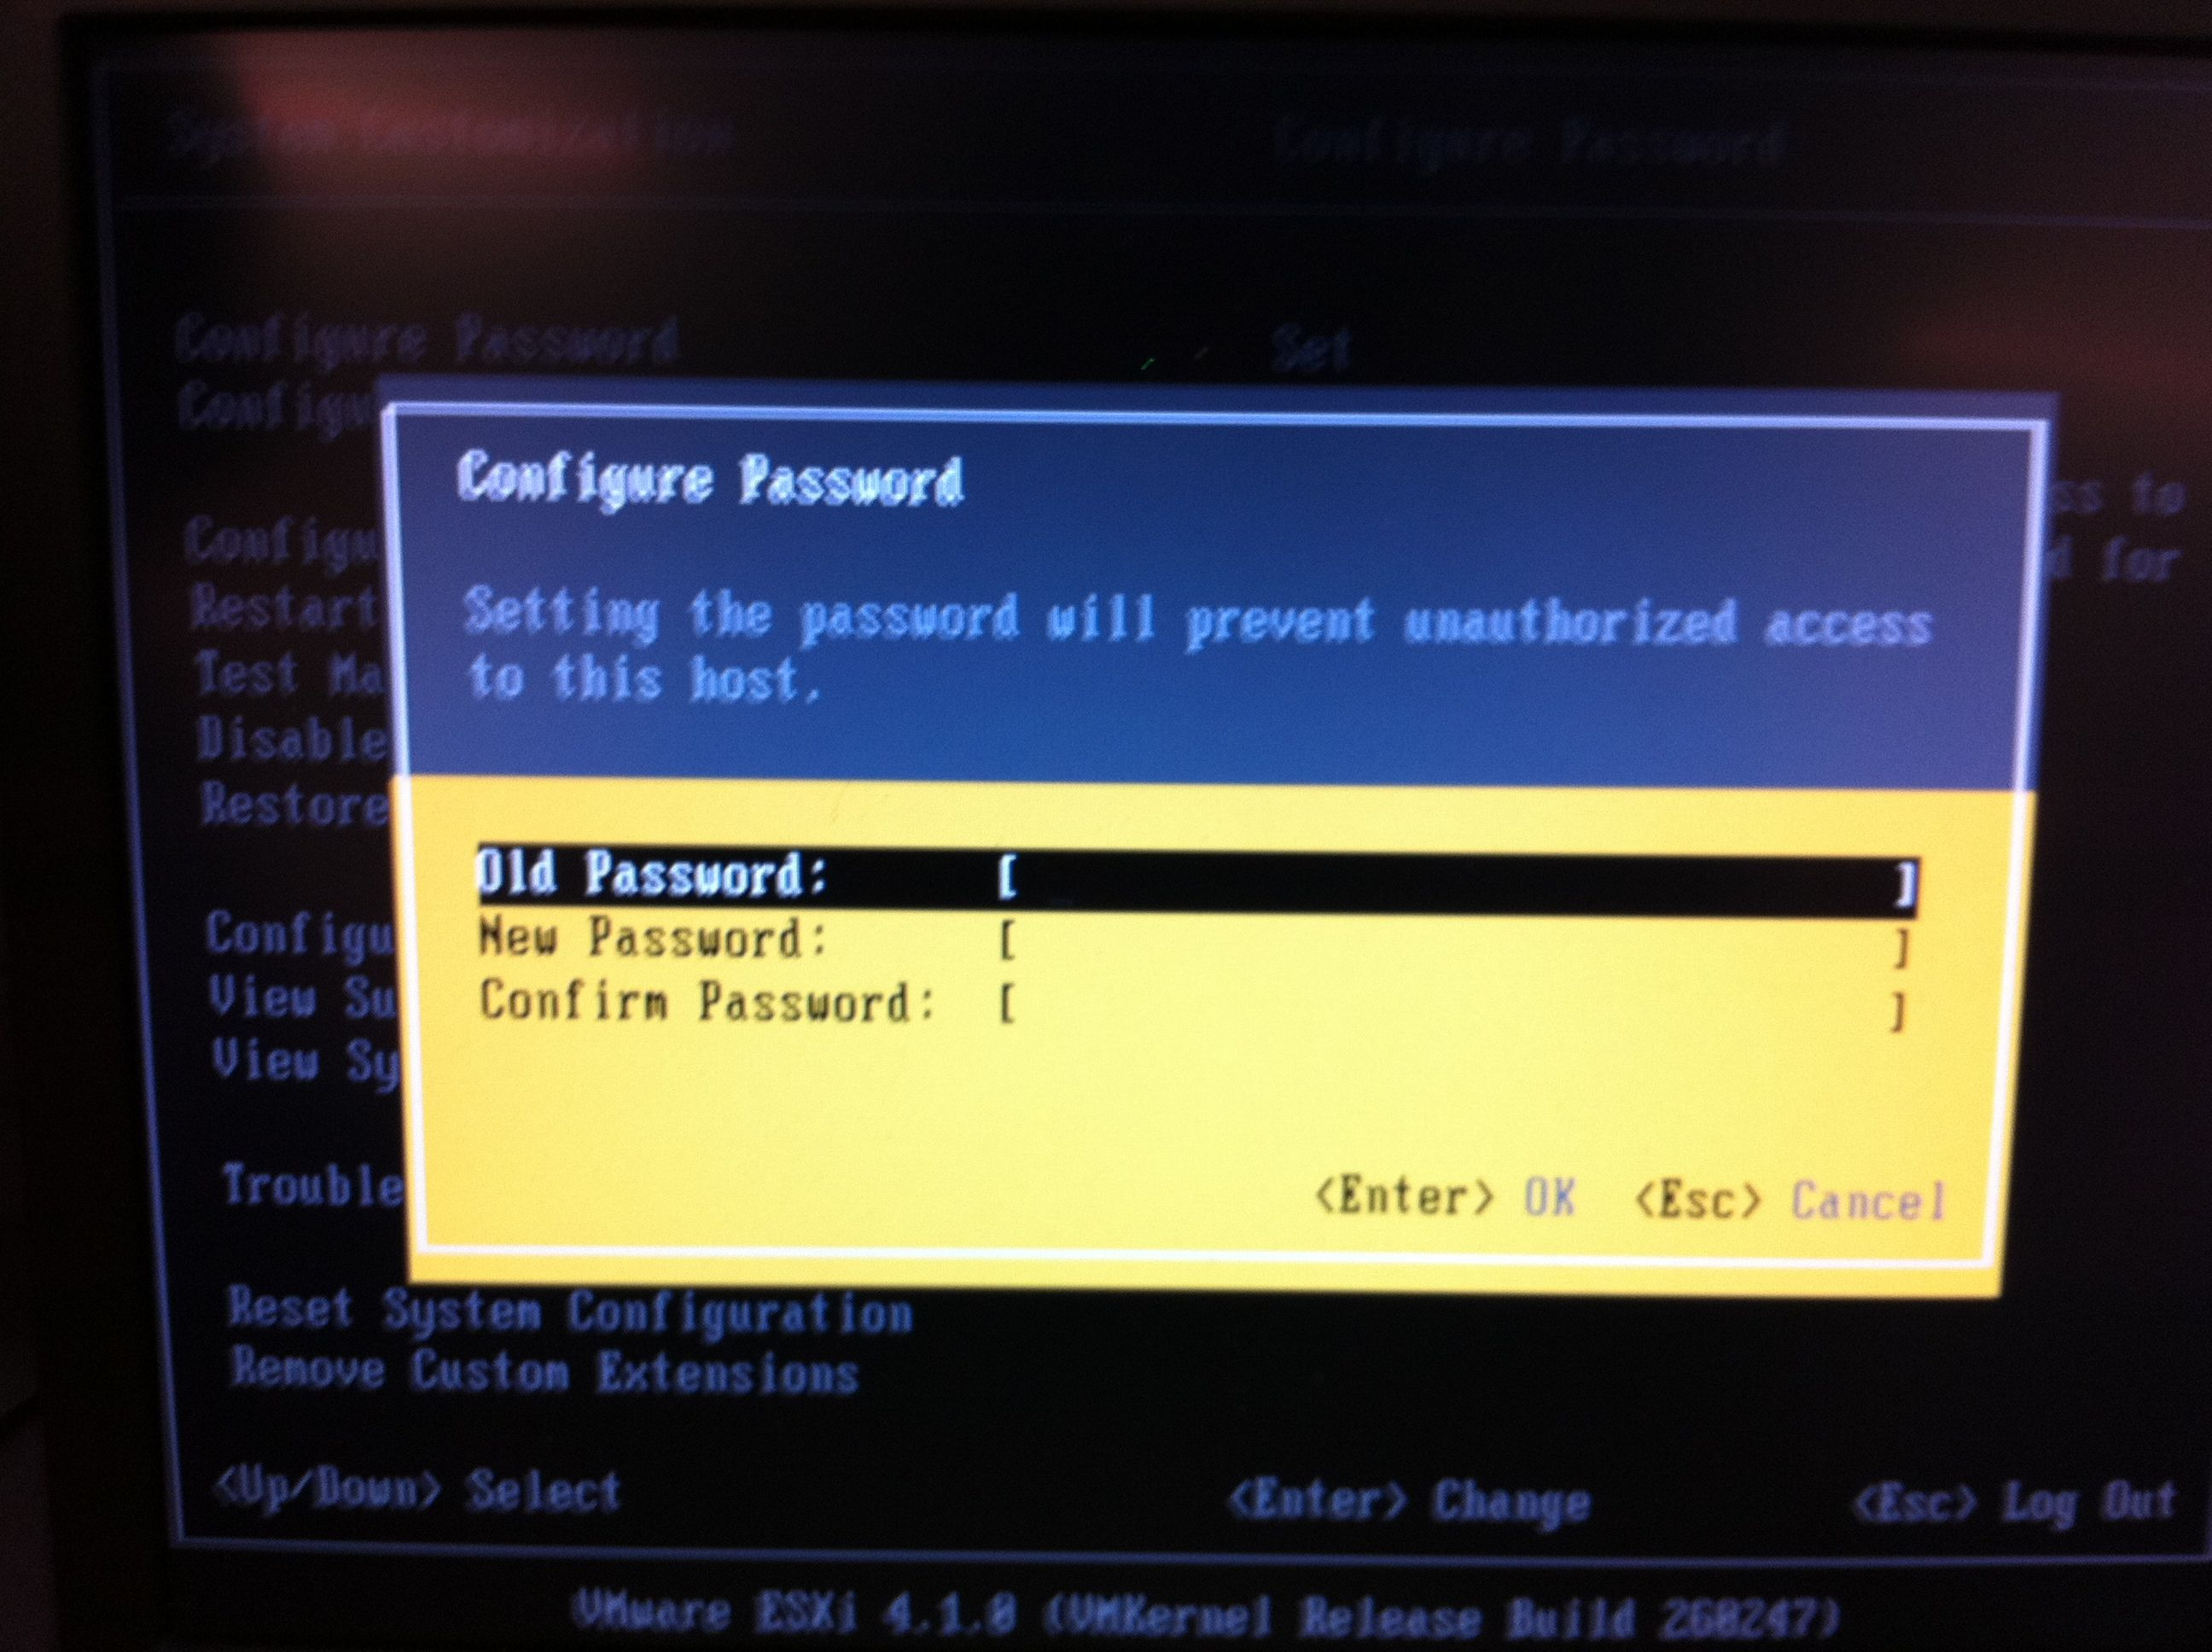
\includegraphics[width=0.5\textwidth]{./pic/esxi_13.jpg}
	\label{fig:esxi_sysconf_pass}
\end{figure}


%---------------
% CREATE VM ON VSPHERE
%---------------
\section{Create a VM with vSphere 4.1}
\label{app:createvm}

Before installing a VM, we need to create it with the vSphere Client. On the item symbolising the ESXi node just right-click and choose "New Virtual Machine...". 

\begin{figure}[ht]
	\caption{vSphere Client - Create VM (Step 1)}
  	\centering
	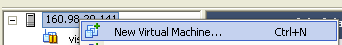
\includegraphics[width=0.5\textwidth]{./pic/createvm_1.png}
	\label{fig:createvm_1}
\end{figure}
\pagebreak


Choose "Typical" configuration and click "Next".
\begin{figure}[ht]
	\caption{vSphere Client - Create VM (Step 2)}
  	\centering
	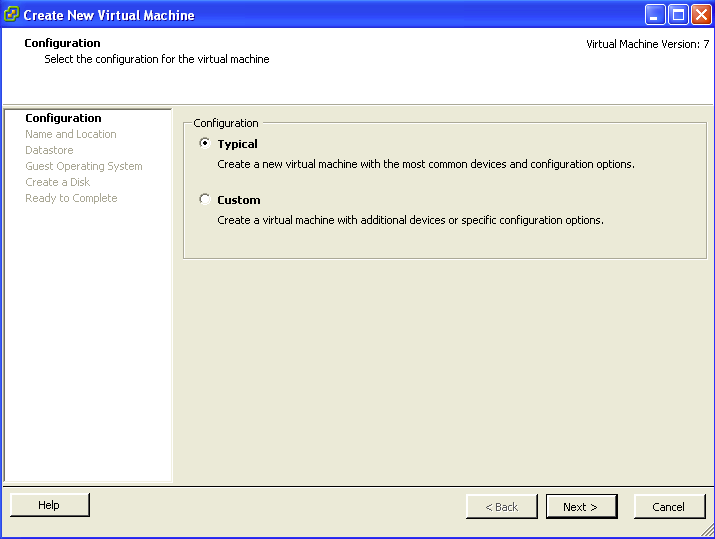
\includegraphics[width=0.5\textwidth]{./pic/createvm_2.png}
	\label{fig:createvm_2}
\end{figure}

Give a name to the VM and click "Next".
\begin{figure}[ht]
	\caption{vSphere Client - Create VM (Step 3)}
  	\centering
	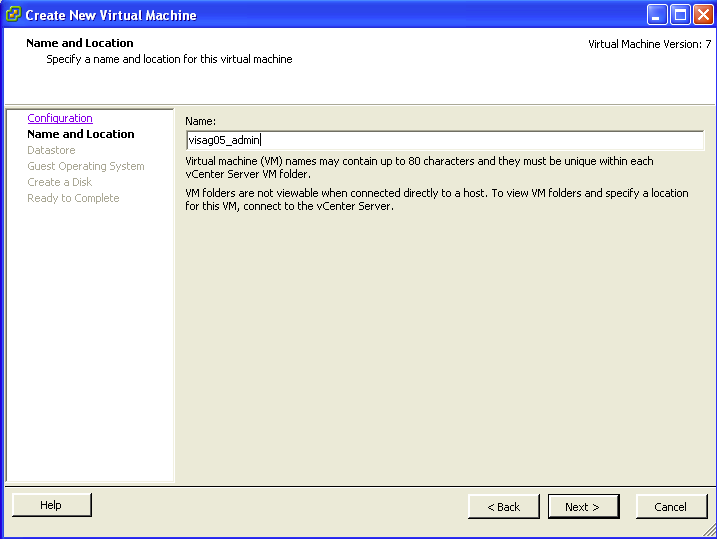
\includegraphics[width=0.5\textwidth]{./pic/createvm_3.png}
	\label{fig:createvm_3}
\end{figure}

\pagebreak
Choose the datastore of destination and click "Next".
\begin{figure}[ht]
	\caption{vSphere Client - Create VM (Step 4)}
  	\centering
	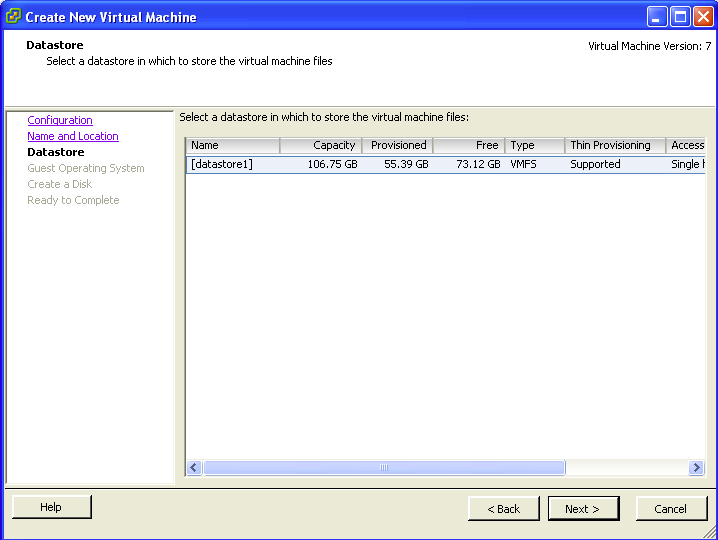
\includegraphics[width=0.5\textwidth]{./pic/createvm_4.png}
	\label{fig:createvm_4}
\end{figure}

Choose the "Operating System" and click "Next".
\begin{figure}[ht]
	\caption{vSphere Client - Create VM (Step 5)}
  	\centering
	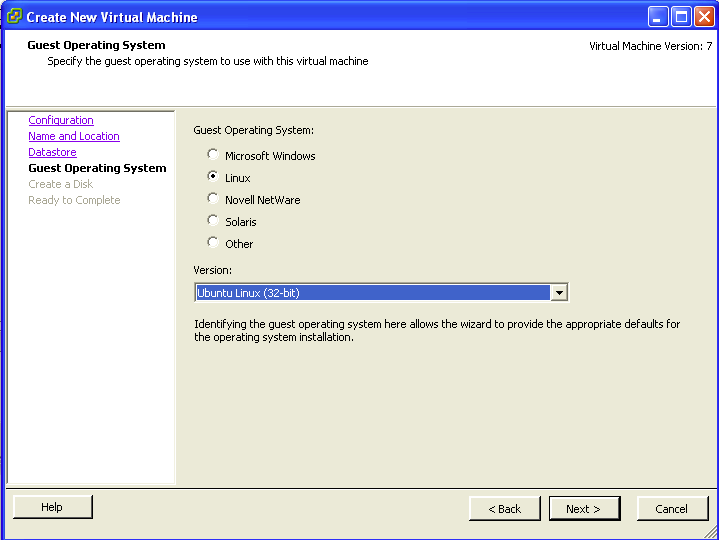
\includegraphics[width=0.5\textwidth]{./pic/createvm_5.png}
	\label{fig:createvm_5}
\end{figure}

\pagebreak
Choose the size of the disk and select "Allocate and commit ..." and click "Next".
\begin{figure}[ht]
	\caption{vSphere Client - Create VM (Step 6)}
  	\centering
	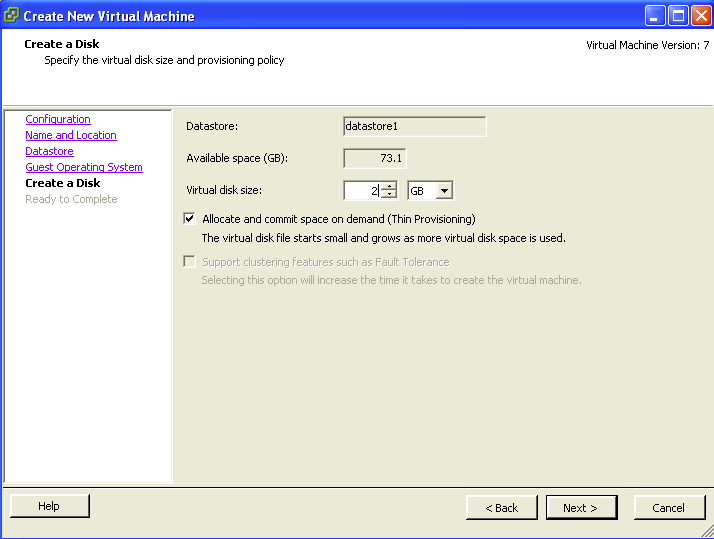
\includegraphics[width=0.5\textwidth]{./pic/createvm_6.png}
	\label{fig:createvm_6}
\end{figure}

Click "Finish", the VM is created and appears in the left-side of the vSphere client. 
\begin{figure}[ht]
	\caption{vSphere Client - Create VM (Step 7)}
  	\centering
	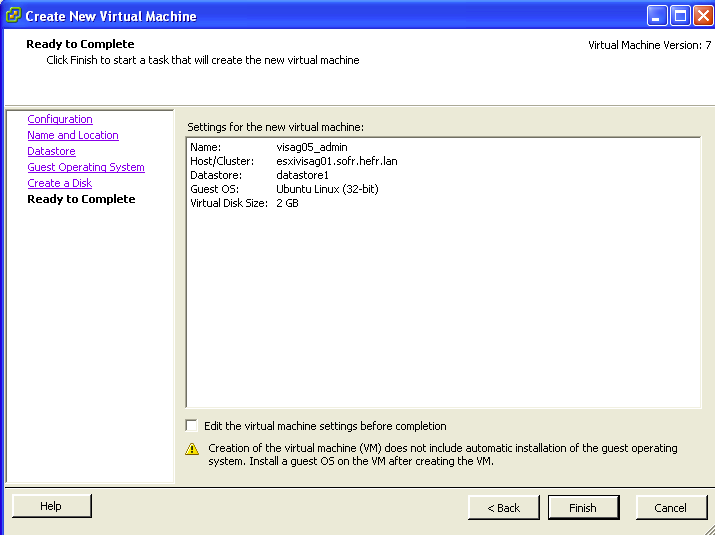
\includegraphics[width=0.5\textwidth]{./pic/createvm_7.png}
	\label{fig:createvm_7}
\end{figure}


\pagebreak
%---------------
% CREATE A SNAPSHOT
%---------------
\section{Create a snapshot of a VM}
\label{app:snap}
The worker VM will be reverted to a snapshot before executing a job. To be able to do this action, we need to create the snapshot of our worker VM in the good state. After installing all the needed elements, you should release the dhcp lease and shutdown the VM. On a Ubuntu OS, use the following command:\s

\begin{lstlisting}
sudo dhclient -r && sudo shutdown -h now
\end{lstlisting}\s

This will remove any IP address information from the snapshot. It is very important to have to shortest revert time possible. Once we have to clean Vm, we can create the snapshot. \s

To create the snapshot, make a right-click on the VM in vSphere Client  and select "Snapshot > Take a snapshot" (see Figure \ref{fig:snap_1}). 

\begin{figure}[ht]
	\caption{vSphere Client - Create Snapshot (Step 1)}
  	\centering
	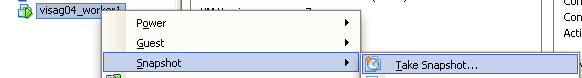
\includegraphics[width=0.5\textwidth]{./pic/snap_1.png}
	\label{fig:snap_1}
\end{figure}


Give a name to the snapshot (this name will be used in the virtual configuration of POP-C++), an optional description and click "Ok" (see Figure \ref{fig:snap_2}). 

\begin{figure}[ht]
	\caption{vSphere Client - Create Snapshot (Step 2)}
  	\centering
	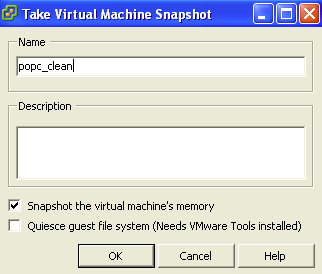
\includegraphics[width=0.5\textwidth]{./pic/snap_2.png}
	\label{fig:snap_2}
\end{figure}

The snapshot will be created (it can take a while to create the snapshot) and the worker will be ready to be used.






\end{document}
